\documentclass[a4paper]{book}
\usepackage{makeidx}
\usepackage{natbib}
\usepackage{graphicx}
\usepackage{multicol}
\usepackage{float}
\usepackage{listings}
\usepackage{color}
\usepackage{ifthen}
\usepackage[table]{xcolor}
\usepackage{textcomp}
\usepackage{alltt}
\usepackage{ifpdf}
\ifpdf
\usepackage[pdftex,
            pagebackref=true,
            colorlinks=true,
            linkcolor=blue,
            unicode
           ]{hyperref}
\else
\usepackage[ps2pdf,
            pagebackref=true,
            colorlinks=true,
            linkcolor=blue,
            unicode
           ]{hyperref}
\usepackage{pspicture}
\fi
\usepackage[utf8]{inputenc}
\usepackage{mathptmx}
\usepackage[scaled=.90]{helvet}
\usepackage{courier}
\usepackage{sectsty}
\usepackage[titles]{tocloft}
\usepackage{doxygen}
\lstset{language=C++,inputencoding=utf8,basicstyle=\footnotesize,breaklines=true,breakatwhitespace=true,tabsize=8,numbers=left }
\makeindex
\setcounter{tocdepth}{3}
\renewcommand{\footrulewidth}{0.4pt}
\renewcommand{\familydefault}{\sfdefault}
\hfuzz=15pt
\setlength{\emergencystretch}{15pt}
\hbadness=750
\tolerance=750
\begin{document}
\hypersetup{pageanchor=false,citecolor=blue}
\begin{titlepage}
\vspace*{7cm}
\begin{center}
{\Large \-Mono \-Odometer \\[1ex]\large 0.\-01 }\\
\vspace*{1cm}
{\large \-Generated by Doxygen 1.7.6.1}\\
\vspace*{0.5cm}
{\small Wed Sep 26 2012 16:02:56}\\
\end{center}
\end{titlepage}
\clearemptydoublepage
\pagenumbering{roman}
\tableofcontents
\clearemptydoublepage
\pagenumbering{arabic}
\hypersetup{pageanchor=true,citecolor=blue}
\chapter{\-Namespace \-Index}
\section{\-Namespace \-List}
\-Here is a list of all namespaces with brief descriptions\-:\begin{DoxyCompactList}
\item\contentsline{section}{\hyperlink{namespaceLRM}{\-L\-R\-M} }{\pageref{namespaceLRM}}{}
\end{DoxyCompactList}

\chapter{\-Class \-Index}
\section{\-Class \-List}
\-Here are the classes, structs, unions and interfaces with brief descriptions\-:\begin{DoxyCompactList}
\item\contentsline{section}{\hyperlink{classLRM_1_1Feature}{\-L\-R\-M\-::\-Feature} }{\pageref{classLRM_1_1Feature}}{}
\item\contentsline{section}{\hyperlink{classLRM_1_1ImageProcessor}{\-L\-R\-M\-::\-Image\-Processor} }{\pageref{classLRM_1_1ImageProcessor}}{}
\item\contentsline{section}{\hyperlink{classLRM_1_1ImageProcessorParameter}{\-L\-R\-M\-::\-Image\-Processor\-Parameter} }{\pageref{classLRM_1_1ImageProcessorParameter}}{}
\item\contentsline{section}{\hyperlink{classLRM_1_1MonoOdometer}{\-L\-R\-M\-::\-Mono\-Odometer} }{\pageref{classLRM_1_1MonoOdometer}}{}
\item\contentsline{section}{\hyperlink{classLRM_1_1MotionProcessor}{\-L\-R\-M\-::\-Motion\-Processor} }{\pageref{classLRM_1_1MotionProcessor}}{}
\item\contentsline{section}{\hyperlink{classLRM_1_1MotionProcessorParameter}{\-L\-R\-M\-::\-Motion\-Processor\-Parameter} }{\pageref{classLRM_1_1MotionProcessorParameter}}{}
\item\contentsline{section}{\hyperlink{classLRM_1_1Parameter}{\-L\-R\-M\-::\-Parameter} }{\pageref{classLRM_1_1Parameter}}{}
\item\contentsline{section}{\hyperlink{classLRM_1_1ROSParameter}{\-L\-R\-M\-::\-R\-O\-S\-Parameter} }{\pageref{classLRM_1_1ROSParameter}}{}
\end{DoxyCompactList}

\chapter{\-File \-Index}
\section{\-File \-List}
\-Here is a list of all files with brief descriptions\-:\begin{DoxyCompactList}
\item\contentsline{section}{include/\hyperlink{feature_8h}{feature.\-h} }{\pageref{feature_8h}}{}
\item\contentsline{section}{include/\hyperlink{frame_8h}{frame.\-h} }{\pageref{frame_8h}}{}
\item\contentsline{section}{include/\hyperlink{mono__odometer_8h}{mono\-\_\-odometer.\-h} }{\pageref{mono__odometer_8h}}{}
\item\contentsline{section}{include/\hyperlink{motion_8h}{motion.\-h} }{\pageref{motion_8h}}{}
\item\contentsline{section}{src/\hyperlink{feature_8cpp}{feature.\-cpp} }{\pageref{feature_8cpp}}{}
\item\contentsline{section}{src/\hyperlink{feature__test_8cpp}{feature\-\_\-test.\-cpp} }{\pageref{feature__test_8cpp}}{}
\item\contentsline{section}{src/\hyperlink{frame_8cpp}{frame.\-cpp} }{\pageref{frame_8cpp}}{}
\item\contentsline{section}{src/\hyperlink{main_8cpp}{main.\-cpp} }{\pageref{main_8cpp}}{}
\item\contentsline{section}{src/\hyperlink{mono__odometer_8cpp}{mono\-\_\-odometer.\-cpp} }{\pageref{mono__odometer_8cpp}}{}
\item\contentsline{section}{src/\hyperlink{motion_8cpp}{motion.\-cpp} }{\pageref{motion_8cpp}}{}
\end{DoxyCompactList}

\chapter{\-Namespace \-Documentation}
\hypertarget{namespaceLRM}{\section{\-L\-R\-M \-Namespace \-Reference}
\label{namespaceLRM}\index{\-L\-R\-M@{\-L\-R\-M}}
}
\subsection*{\-Classes}
\begin{DoxyCompactItemize}
\item 
class \hyperlink{classLRM_1_1Feature}{\-Feature}
\item 
class \hyperlink{classLRM_1_1ImageProcessorParameter}{\-Image\-Processor\-Parameter}
\item 
class \hyperlink{classLRM_1_1ImageProcessor}{\-Image\-Processor}
\item 
class \hyperlink{classLRM_1_1ROSParameter}{\-R\-O\-S\-Parameter}
\item 
class \hyperlink{classLRM_1_1MonoOdometer}{\-Mono\-Odometer}
\item 
class \hyperlink{classLRM_1_1MotionProcessorParameter}{\-Motion\-Processor\-Parameter}
\item 
class \hyperlink{classLRM_1_1MotionProcessor}{\-Motion\-Processor}
\item 
class \hyperlink{classLRM_1_1Parameter}{\-Parameter}
\end{DoxyCompactItemize}
\subsection*{\-Enumerations}
\begin{DoxyCompactItemize}
\item 
enum \hyperlink{namespaceLRM_a8eb6956b84fb7d27bce5af771937794f}{feature\-\_\-t} \{ \*
\hyperlink{namespaceLRM_a8eb6956b84fb7d27bce5af771937794fa8e3a2d26370c85d7adb97cbbd40abc72}{\-S\-H\-I\-\_\-\-T\-O\-M\-A\-S\-I}, 
\hyperlink{namespaceLRM_a8eb6956b84fb7d27bce5af771937794fa82f8a835c4a989b4beddacd8082dc75d}{\-H\-A\-R\-R\-I\-S}, 
\hyperlink{namespaceLRM_a8eb6956b84fb7d27bce5af771937794fa7c70db53c6ef257d06ad41cd33ea8c42}{\-O\-R\-B}, 
\hyperlink{namespaceLRM_a8eb6956b84fb7d27bce5af771937794fa68bc6d3980e55f5e357855916be07ab9}{\-F\-A\-S\-T}, 
\*
\hyperlink{namespaceLRM_a8eb6956b84fb7d27bce5af771937794fabace5d3a329784433515af3067c3e9d9}{\-S\-U\-R\-F}, 
\hyperlink{namespaceLRM_a8eb6956b84fb7d27bce5af771937794fab88abdea089ea29c5224698eb2215891}{\-S\-I\-F\-T}, 
\hyperlink{namespaceLRM_a8eb6956b84fb7d27bce5af771937794faa8a3283e5421c1218d8238e56c80a104}{\-N\-O\-\_\-\-F\-E\-A\-T\-U\-R\-E}
 \}
\begin{DoxyCompactList}\small\item\em \-Types of possible features. \end{DoxyCompactList}\item 
enum \hyperlink{namespaceLRM_ad31d475a7f32e1bd208beb34aabc6fa9}{descriptor\-\_\-t} \{ \hyperlink{namespaceLRM_ad31d475a7f32e1bd208beb34aabc6fa9a1e43a18048d2fc5fc782f2eebce0d585}{\-S\-S\-D}
 \}
\begin{DoxyCompactList}\small\item\em \-Types of possible descriptors. \end{DoxyCompactList}\end{DoxyCompactItemize}


\subsection{\-Enumeration \-Type \-Documentation}
\hypertarget{namespaceLRM_ad31d475a7f32e1bd208beb34aabc6fa9}{\index{\-L\-R\-M@{\-L\-R\-M}!descriptor\-\_\-t@{descriptor\-\_\-t}}
\index{descriptor\-\_\-t@{descriptor\-\_\-t}!LRM@{\-L\-R\-M}}
\subsubsection[{descriptor\-\_\-t}]{\setlength{\rightskip}{0pt plus 5cm}enum {\bf \-L\-R\-M\-::descriptor\-\_\-t}}}\label{namespaceLRM_ad31d475a7f32e1bd208beb34aabc6fa9}


\-Types of possible descriptors. 

\begin{Desc}
\item[\-Enumerator\-: ]\par
\begin{description}
\index{\-S\-S\-D@{\-S\-S\-D}!\-L\-R\-M@{\-L\-R\-M}}\index{\-L\-R\-M@{\-L\-R\-M}!\-S\-S\-D@{\-S\-S\-D}}\item[{\em 
\hypertarget{namespaceLRM_ad31d475a7f32e1bd208beb34aabc6fa9a1e43a18048d2fc5fc782f2eebce0d585}{\-S\-S\-D}\label{namespaceLRM_ad31d475a7f32e1bd208beb34aabc6fa9a1e43a18048d2fc5fc782f2eebce0d585}
}]\end{description}
\end{Desc}

\hypertarget{namespaceLRM_a8eb6956b84fb7d27bce5af771937794f}{\index{\-L\-R\-M@{\-L\-R\-M}!feature\-\_\-t@{feature\-\_\-t}}
\index{feature\-\_\-t@{feature\-\_\-t}!LRM@{\-L\-R\-M}}
\subsubsection[{feature\-\_\-t}]{\setlength{\rightskip}{0pt plus 5cm}enum {\bf \-L\-R\-M\-::feature\-\_\-t}}}\label{namespaceLRM_a8eb6956b84fb7d27bce5af771937794f}


\-Types of possible features. 

\begin{Desc}
\item[\-Enumerator\-: ]\par
\begin{description}
\index{\-S\-H\-I\-\_\-\-T\-O\-M\-A\-S\-I@{\-S\-H\-I\-\_\-\-T\-O\-M\-A\-S\-I}!\-L\-R\-M@{\-L\-R\-M}}\index{\-L\-R\-M@{\-L\-R\-M}!\-S\-H\-I\-\_\-\-T\-O\-M\-A\-S\-I@{\-S\-H\-I\-\_\-\-T\-O\-M\-A\-S\-I}}\item[{\em 
\hypertarget{namespaceLRM_a8eb6956b84fb7d27bce5af771937794fa8e3a2d26370c85d7adb97cbbd40abc72}{\-S\-H\-I\-\_\-\-T\-O\-M\-A\-S\-I}\label{namespaceLRM_a8eb6956b84fb7d27bce5af771937794fa8e3a2d26370c85d7adb97cbbd40abc72}
}]\index{\-H\-A\-R\-R\-I\-S@{\-H\-A\-R\-R\-I\-S}!\-L\-R\-M@{\-L\-R\-M}}\index{\-L\-R\-M@{\-L\-R\-M}!\-H\-A\-R\-R\-I\-S@{\-H\-A\-R\-R\-I\-S}}\item[{\em 
\hypertarget{namespaceLRM_a8eb6956b84fb7d27bce5af771937794fa82f8a835c4a989b4beddacd8082dc75d}{\-H\-A\-R\-R\-I\-S}\label{namespaceLRM_a8eb6956b84fb7d27bce5af771937794fa82f8a835c4a989b4beddacd8082dc75d}
}]\index{\-O\-R\-B@{\-O\-R\-B}!\-L\-R\-M@{\-L\-R\-M}}\index{\-L\-R\-M@{\-L\-R\-M}!\-O\-R\-B@{\-O\-R\-B}}\item[{\em 
\hypertarget{namespaceLRM_a8eb6956b84fb7d27bce5af771937794fa7c70db53c6ef257d06ad41cd33ea8c42}{\-O\-R\-B}\label{namespaceLRM_a8eb6956b84fb7d27bce5af771937794fa7c70db53c6ef257d06ad41cd33ea8c42}
}]\index{\-F\-A\-S\-T@{\-F\-A\-S\-T}!\-L\-R\-M@{\-L\-R\-M}}\index{\-L\-R\-M@{\-L\-R\-M}!\-F\-A\-S\-T@{\-F\-A\-S\-T}}\item[{\em 
\hypertarget{namespaceLRM_a8eb6956b84fb7d27bce5af771937794fa68bc6d3980e55f5e357855916be07ab9}{\-F\-A\-S\-T}\label{namespaceLRM_a8eb6956b84fb7d27bce5af771937794fa68bc6d3980e55f5e357855916be07ab9}
}]\index{\-S\-U\-R\-F@{\-S\-U\-R\-F}!\-L\-R\-M@{\-L\-R\-M}}\index{\-L\-R\-M@{\-L\-R\-M}!\-S\-U\-R\-F@{\-S\-U\-R\-F}}\item[{\em 
\hypertarget{namespaceLRM_a8eb6956b84fb7d27bce5af771937794fabace5d3a329784433515af3067c3e9d9}{\-S\-U\-R\-F}\label{namespaceLRM_a8eb6956b84fb7d27bce5af771937794fabace5d3a329784433515af3067c3e9d9}
}]\index{\-S\-I\-F\-T@{\-S\-I\-F\-T}!\-L\-R\-M@{\-L\-R\-M}}\index{\-L\-R\-M@{\-L\-R\-M}!\-S\-I\-F\-T@{\-S\-I\-F\-T}}\item[{\em 
\hypertarget{namespaceLRM_a8eb6956b84fb7d27bce5af771937794fab88abdea089ea29c5224698eb2215891}{\-S\-I\-F\-T}\label{namespaceLRM_a8eb6956b84fb7d27bce5af771937794fab88abdea089ea29c5224698eb2215891}
}]\index{\-N\-O\-\_\-\-F\-E\-A\-T\-U\-R\-E@{\-N\-O\-\_\-\-F\-E\-A\-T\-U\-R\-E}!\-L\-R\-M@{\-L\-R\-M}}\index{\-L\-R\-M@{\-L\-R\-M}!\-N\-O\-\_\-\-F\-E\-A\-T\-U\-R\-E@{\-N\-O\-\_\-\-F\-E\-A\-T\-U\-R\-E}}\item[{\em 
\hypertarget{namespaceLRM_a8eb6956b84fb7d27bce5af771937794faa8a3283e5421c1218d8238e56c80a104}{\-N\-O\-\_\-\-F\-E\-A\-T\-U\-R\-E}\label{namespaceLRM_a8eb6956b84fb7d27bce5af771937794faa8a3283e5421c1218d8238e56c80a104}
}]\end{description}
\end{Desc}


\chapter{\-Class \-Documentation}
\hypertarget{classLRM_1_1Descriptor}{\section{\-L\-R\-M\-:\-:\-Descriptor \-Class \-Reference}
\label{classLRM_1_1Descriptor}\index{\-L\-R\-M\-::\-Descriptor@{\-L\-R\-M\-::\-Descriptor}}
}


{\ttfamily \#include $<$feature.\-h$>$}



\-The documentation for this class was generated from the following file\-:\begin{DoxyCompactItemize}
\item 
include/\hyperlink{feature_8h}{feature.\-h}\end{DoxyCompactItemize}

\hypertarget{classLRM_1_1Feature}{\section{\-L\-R\-M\-:\-:\-Feature \-Class \-Reference}
\label{classLRM_1_1Feature}\index{\-L\-R\-M\-::\-Feature@{\-L\-R\-M\-::\-Feature}}
}


{\ttfamily \#include $<$core.\-h$>$}

\subsection*{\-Static \-Public \-Member \-Functions}
\begin{DoxyCompactItemize}
\item 
static \hyperlink{namespaceLRM_a8eb6956b84fb7d27bce5af771937794f}{feature\-\_\-t} \hyperlink{classLRM_1_1Feature_ad9c5e3c4db26357168ba34ae1f3e566c}{get\-Feature\-By\-Name} (std\-::string feature\-\_\-name)
\end{DoxyCompactItemize}


\subsection{\-Member \-Function \-Documentation}
\hypertarget{classLRM_1_1Feature_ad9c5e3c4db26357168ba34ae1f3e566c}{\index{\-L\-R\-M\-::\-Feature@{\-L\-R\-M\-::\-Feature}!get\-Feature\-By\-Name@{get\-Feature\-By\-Name}}
\index{get\-Feature\-By\-Name@{get\-Feature\-By\-Name}!LRM::Feature@{\-L\-R\-M\-::\-Feature}}
\subsubsection[{get\-Feature\-By\-Name}]{\setlength{\rightskip}{0pt plus 5cm}static {\bf feature\-\_\-t} {\bf \-L\-R\-M\-::\-Feature\-::get\-Feature\-By\-Name} (
\begin{DoxyParamCaption}
\item[{std\-::string}]{feature\-\_\-name}
\end{DoxyParamCaption}
)\hspace{0.3cm}{\ttfamily  \mbox{[}inline, static\mbox{]}}}}\label{classLRM_1_1Feature_ad9c5e3c4db26357168ba34ae1f3e566c}


\-The documentation for this class was generated from the following file\-:\begin{DoxyCompactItemize}
\item 
include/\hyperlink{core_8h}{core.\-h}\end{DoxyCompactItemize}

\hypertarget{classLRM_1_1Frame}{\section{\-L\-R\-M\-:\-:\-Frame \-Class \-Reference}
\label{classLRM_1_1Frame}\index{\-L\-R\-M\-::\-Frame@{\-L\-R\-M\-::\-Frame}}
}


{\ttfamily \#include $<$frame.\-h$>$}

\subsection*{\-Public \-Member \-Functions}
\begin{DoxyCompactItemize}
\item 
\hyperlink{classLRM_1_1Frame_a636777ddefb4bdd602fba813ed415d7c}{\-Frame} (ros\-::\-Node\-Handle nh)
\item 
virtual \hyperlink{classLRM_1_1Frame_a4bc612464eb751bbefba26e7f9e6342f}{$\sim$\-Frame} ()
\item 
void \hyperlink{classLRM_1_1Frame_a9358dbaa793683ab3410b01f322f7a2a}{extract} ()
\end{DoxyCompactItemize}
\subsection*{\-Static \-Public \-Member \-Functions}
\begin{DoxyCompactItemize}
\item 
static void \hyperlink{classLRM_1_1Frame_a32abb5b5830bb7656b7234fe5ba92ef3}{match} ()
\end{DoxyCompactItemize}
\subsection*{\-Private \-Member \-Functions}
\begin{DoxyCompactItemize}
\item 
int \hyperlink{classLRM_1_1Frame_a0cbaae54e9e1ff08532b57b076a0e61e}{corner\-Detector} (cv\-::\-Mat src, \hyperlink{namespaceLRM_a8eb6956b84fb7d27bce5af771937794f}{feature\-\_\-t} \hyperlink{classLRM_1_1Frame_a4984e53e358e726cbf67a55e1cb4f01a}{f\-Type})
\end{DoxyCompactItemize}
\subsection*{\-Private \-Attributes}
\begin{DoxyCompactItemize}
\item 
\hyperlink{namespaceLRM_a8eb6956b84fb7d27bce5af771937794f}{feature\-\_\-t} \hyperlink{classLRM_1_1Frame_a4984e53e358e726cbf67a55e1cb4f01a}{f\-Type}
\begin{DoxyCompactList}\small\item\em \-Type of features detected. \end{DoxyCompactList}\item 
\hyperlink{namespaceLRM_ad31d475a7f32e1bd208beb34aabc6fa9}{descriptor\-\_\-t} \hyperlink{classLRM_1_1Frame_abf992f7a74b18ad8eb8baeab274e2a1b}{d\-Type}
\begin{DoxyCompactList}\small\item\em \-Type of features descriptors used. \end{DoxyCompactList}\item 
std\-::vector$<$ \hyperlink{classLRM_1_1Feature}{\-Feature} $>$ \hyperlink{classLRM_1_1Frame_ad52722b8e517f54086604ff8c3d524ad}{feat\-List}
\begin{DoxyCompactList}\small\item\em \-Detected features list. \end{DoxyCompactList}\item 
std\-::vector$<$ \hyperlink{classLRM_1_1Descriptor}{\-Descriptor} $>$ \hyperlink{classLRM_1_1Frame_ad7f4cd20847b05393d8c0e49e4a07374}{desc\-List}
\begin{DoxyCompactList}\small\item\em \-Detected features descriptors list. \end{DoxyCompactList}\item 
image\-\_\-transport\-::\-Image\-Transport \hyperlink{classLRM_1_1Frame_a9a85162296d550daca6fcf0e39a34f5a}{it}
\begin{DoxyCompactList}\small\item\em \-Image node handler. \end{DoxyCompactList}\item 
image\-\_\-transport\-::\-Subscriber \hyperlink{classLRM_1_1Frame_afde5ec8c81b21aa924f5b054b31e055a}{sub}
\begin{DoxyCompactList}\small\item\em \-Image subscriber. \end{DoxyCompactList}\item 
image\-\_\-transport\-::\-Publisher \hyperlink{classLRM_1_1Frame_a70a2be50521677bd21c4853ce2ccb0f4}{pub}
\begin{DoxyCompactList}\small\item\em \-Image publisher. \end{DoxyCompactList}\end{DoxyCompactItemize}


\subsection{\-Constructor \& \-Destructor \-Documentation}
\hypertarget{classLRM_1_1Frame_a636777ddefb4bdd602fba813ed415d7c}{\index{\-L\-R\-M\-::\-Frame@{\-L\-R\-M\-::\-Frame}!\-Frame@{\-Frame}}
\index{\-Frame@{\-Frame}!LRM::Frame@{\-L\-R\-M\-::\-Frame}}
\subsubsection[{\-Frame}]{\setlength{\rightskip}{0pt plus 5cm}{\bf \-L\-R\-M\-::\-Frame\-::\-Frame} (
\begin{DoxyParamCaption}
\item[{ros\-::\-Node\-Handle}]{nh}
\end{DoxyParamCaption}
)}}\label{classLRM_1_1Frame_a636777ddefb4bdd602fba813ed415d7c}
\hyperlink{classLRM_1_1Frame}{\-Frame} \-Constructor\-: \-Instantiates a new frame. \-The \hyperlink{classLRM_1_1Frame}{\-Frame} class subscribes a frame from a camera and process it identifying features and descriptors. \-Also responsible for the match of the features over other frames.


\begin{DoxyParams}[1]{\-Parameters}
\mbox{\tt in}  & {\em nh} & \-Node handle of the node of the monocular odometer. \\
\hline
\end{DoxyParams}
\hypertarget{classLRM_1_1Frame_a4bc612464eb751bbefba26e7f9e6342f}{\index{\-L\-R\-M\-::\-Frame@{\-L\-R\-M\-::\-Frame}!$\sim$\-Frame@{$\sim$\-Frame}}
\index{$\sim$\-Frame@{$\sim$\-Frame}!LRM::Frame@{\-L\-R\-M\-::\-Frame}}
\subsubsection[{$\sim$\-Frame}]{\setlength{\rightskip}{0pt plus 5cm}{\bf \-L\-R\-M\-::\-Frame\-::$\sim$\-Frame} (
\begin{DoxyParamCaption}
{}
\end{DoxyParamCaption}
)\hspace{0.3cm}{\ttfamily  \mbox{[}virtual\mbox{]}}}}\label{classLRM_1_1Frame_a4bc612464eb751bbefba26e7f9e6342f}


\subsection{\-Member \-Function \-Documentation}
\hypertarget{classLRM_1_1Frame_a0cbaae54e9e1ff08532b57b076a0e61e}{\index{\-L\-R\-M\-::\-Frame@{\-L\-R\-M\-::\-Frame}!corner\-Detector@{corner\-Detector}}
\index{corner\-Detector@{corner\-Detector}!LRM::Frame@{\-L\-R\-M\-::\-Frame}}
\subsubsection[{corner\-Detector}]{\setlength{\rightskip}{0pt plus 5cm}int {\bf \-L\-R\-M\-::\-Frame\-::corner\-Detector} (
\begin{DoxyParamCaption}
\item[{cv\-::\-Mat}]{src, }
\item[{{\bf feature\-\_\-t}}]{f\-Type}
\end{DoxyParamCaption}
)\hspace{0.3cm}{\ttfamily  \mbox{[}private\mbox{]}}}}\label{classLRM_1_1Frame_a0cbaae54e9e1ff08532b57b076a0e61e}
\-Method corner\-Detector\-: \hyperlink{classLRM_1_1Feature}{\-Feature} detection using either \-Harris or \-Shi-\/\-Tomasi methods for corner detection.


\begin{DoxyParams}[1]{\-Parameters}
\mbox{\tt in}  & {\em src} & \-Input image \\
\hline
\mbox{\tt in}  & {\em f\-Type} & \hyperlink{classLRM_1_1Feature}{\-Feature} type. \-Either \-H\-A\-R\-R\-I\-S or \-S\-H\-I\-\_\-\-T\-O\-M\-A\-S\-I. \\
\hline
\end{DoxyParams}
\hypertarget{classLRM_1_1Frame_a9358dbaa793683ab3410b01f322f7a2a}{\index{\-L\-R\-M\-::\-Frame@{\-L\-R\-M\-::\-Frame}!extract@{extract}}
\index{extract@{extract}!LRM::Frame@{\-L\-R\-M\-::\-Frame}}
\subsubsection[{extract}]{\setlength{\rightskip}{0pt plus 5cm}void {\bf \-L\-R\-M\-::\-Frame\-::extract} (
\begin{DoxyParamCaption}
{}
\end{DoxyParamCaption}
)}}\label{classLRM_1_1Frame_a9358dbaa793683ab3410b01f322f7a2a}
\-Method extract\-: \-The method extract is responsible to detect to extract the features of a input image. \hypertarget{classLRM_1_1Frame_a32abb5b5830bb7656b7234fe5ba92ef3}{\index{\-L\-R\-M\-::\-Frame@{\-L\-R\-M\-::\-Frame}!match@{match}}
\index{match@{match}!LRM::Frame@{\-L\-R\-M\-::\-Frame}}
\subsubsection[{match}]{\setlength{\rightskip}{0pt plus 5cm}static void {\bf \-L\-R\-M\-::\-Frame\-::match} (
\begin{DoxyParamCaption}
{}
\end{DoxyParamCaption}
)\hspace{0.3cm}{\ttfamily  \mbox{[}static\mbox{]}}}}\label{classLRM_1_1Frame_a32abb5b5830bb7656b7234fe5ba92ef3}


\subsection{\-Member \-Data \-Documentation}
\hypertarget{classLRM_1_1Frame_ad7f4cd20847b05393d8c0e49e4a07374}{\index{\-L\-R\-M\-::\-Frame@{\-L\-R\-M\-::\-Frame}!desc\-List@{desc\-List}}
\index{desc\-List@{desc\-List}!LRM::Frame@{\-L\-R\-M\-::\-Frame}}
\subsubsection[{desc\-List}]{\setlength{\rightskip}{0pt plus 5cm}std\-::vector$<${\bf \-Descriptor}$>$ {\bf \-L\-R\-M\-::\-Frame\-::desc\-List}\hspace{0.3cm}{\ttfamily  \mbox{[}private\mbox{]}}}}\label{classLRM_1_1Frame_ad7f4cd20847b05393d8c0e49e4a07374}


\-Detected features descriptors list. 

\hypertarget{classLRM_1_1Frame_abf992f7a74b18ad8eb8baeab274e2a1b}{\index{\-L\-R\-M\-::\-Frame@{\-L\-R\-M\-::\-Frame}!d\-Type@{d\-Type}}
\index{d\-Type@{d\-Type}!LRM::Frame@{\-L\-R\-M\-::\-Frame}}
\subsubsection[{d\-Type}]{\setlength{\rightskip}{0pt plus 5cm}{\bf descriptor\-\_\-t} {\bf \-L\-R\-M\-::\-Frame\-::d\-Type}\hspace{0.3cm}{\ttfamily  \mbox{[}private\mbox{]}}}}\label{classLRM_1_1Frame_abf992f7a74b18ad8eb8baeab274e2a1b}


\-Type of features descriptors used. 

\hypertarget{classLRM_1_1Frame_ad52722b8e517f54086604ff8c3d524ad}{\index{\-L\-R\-M\-::\-Frame@{\-L\-R\-M\-::\-Frame}!feat\-List@{feat\-List}}
\index{feat\-List@{feat\-List}!LRM::Frame@{\-L\-R\-M\-::\-Frame}}
\subsubsection[{feat\-List}]{\setlength{\rightskip}{0pt plus 5cm}std\-::vector$<${\bf \-Feature}$>$ {\bf \-L\-R\-M\-::\-Frame\-::feat\-List}\hspace{0.3cm}{\ttfamily  \mbox{[}private\mbox{]}}}}\label{classLRM_1_1Frame_ad52722b8e517f54086604ff8c3d524ad}


\-Detected features list. 

\hypertarget{classLRM_1_1Frame_a4984e53e358e726cbf67a55e1cb4f01a}{\index{\-L\-R\-M\-::\-Frame@{\-L\-R\-M\-::\-Frame}!f\-Type@{f\-Type}}
\index{f\-Type@{f\-Type}!LRM::Frame@{\-L\-R\-M\-::\-Frame}}
\subsubsection[{f\-Type}]{\setlength{\rightskip}{0pt plus 5cm}{\bf feature\-\_\-t} {\bf \-L\-R\-M\-::\-Frame\-::f\-Type}\hspace{0.3cm}{\ttfamily  \mbox{[}private\mbox{]}}}}\label{classLRM_1_1Frame_a4984e53e358e726cbf67a55e1cb4f01a}


\-Type of features detected. 

\hypertarget{classLRM_1_1Frame_a9a85162296d550daca6fcf0e39a34f5a}{\index{\-L\-R\-M\-::\-Frame@{\-L\-R\-M\-::\-Frame}!it@{it}}
\index{it@{it}!LRM::Frame@{\-L\-R\-M\-::\-Frame}}
\subsubsection[{it}]{\setlength{\rightskip}{0pt plus 5cm}image\-\_\-transport\-::\-Image\-Transport {\bf \-L\-R\-M\-::\-Frame\-::it}\hspace{0.3cm}{\ttfamily  \mbox{[}private\mbox{]}}}}\label{classLRM_1_1Frame_a9a85162296d550daca6fcf0e39a34f5a}


\-Image node handler. 

\hypertarget{classLRM_1_1Frame_a70a2be50521677bd21c4853ce2ccb0f4}{\index{\-L\-R\-M\-::\-Frame@{\-L\-R\-M\-::\-Frame}!pub@{pub}}
\index{pub@{pub}!LRM::Frame@{\-L\-R\-M\-::\-Frame}}
\subsubsection[{pub}]{\setlength{\rightskip}{0pt plus 5cm}image\-\_\-transport\-::\-Publisher {\bf \-L\-R\-M\-::\-Frame\-::pub}\hspace{0.3cm}{\ttfamily  \mbox{[}private\mbox{]}}}}\label{classLRM_1_1Frame_a70a2be50521677bd21c4853ce2ccb0f4}


\-Image publisher. 

\hypertarget{classLRM_1_1Frame_afde5ec8c81b21aa924f5b054b31e055a}{\index{\-L\-R\-M\-::\-Frame@{\-L\-R\-M\-::\-Frame}!sub@{sub}}
\index{sub@{sub}!LRM::Frame@{\-L\-R\-M\-::\-Frame}}
\subsubsection[{sub}]{\setlength{\rightskip}{0pt plus 5cm}image\-\_\-transport\-::\-Subscriber {\bf \-L\-R\-M\-::\-Frame\-::sub}\hspace{0.3cm}{\ttfamily  \mbox{[}private\mbox{]}}}}\label{classLRM_1_1Frame_afde5ec8c81b21aa924f5b054b31e055a}


\-Image subscriber. 



\-The documentation for this class was generated from the following files\-:\begin{DoxyCompactItemize}
\item 
include/\hyperlink{frame_8h}{frame.\-h}\item 
src/\hyperlink{frame_8cpp}{frame.\-cpp}\end{DoxyCompactItemize}

\hypertarget{classLRM_1_1MonoOdometer}{\section{\-L\-R\-M\-:\-:\-Mono\-Odometer \-Class \-Reference}
\label{classLRM_1_1MonoOdometer}\index{\-L\-R\-M\-::\-Mono\-Odometer@{\-L\-R\-M\-::\-Mono\-Odometer}}
}


{\ttfamily \#include $<$mono\-\_\-odometer.\-h$>$}



\-Collaboration diagram for \-L\-R\-M\-:\-:\-Mono\-Odometer\-:\nopagebreak
\begin{figure}[H]
\begin{center}
\leavevmode
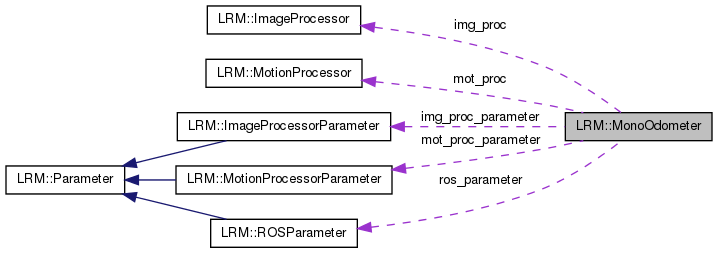
\includegraphics[width=350pt]{classLRM_1_1MonoOdometer__coll__graph}
\end{center}
\end{figure}
\subsection*{\-Public \-Member \-Functions}
\begin{DoxyCompactItemize}
\item 
\hyperlink{classLRM_1_1MonoOdometer_a1ea1f329885905fcab0e3f790253df9d}{\-Mono\-Odometer} ()
\item 
\hyperlink{classLRM_1_1MonoOdometer_ae849abdcd3e0b49be6b1672b292c86ba}{\-Mono\-Odometer} (ros\-::\-Node\-Handle \&nh, image\-\_\-transport\-::\-Image\-Transport \&it)
\begin{DoxyCompactList}\small\item\em \-The constructor of the \-Mono \-Odometer class. \-Captures and process a new frame and estimates the momentaneous motion. \end{DoxyCompactList}\item 
\hyperlink{classLRM_1_1MonoOdometer_aadca97effbd3970022f8fdfa42c1177b}{$\sim$\-Mono\-Odometer} ()
\item 
void \hyperlink{classLRM_1_1MonoOdometer_a7205e77893b1f9d4c37de616519ef5ed}{\-Image\-Callback} (const sensor\-\_\-msgs\-::\-Image\-Const\-Ptr \&msg)
\begin{DoxyCompactList}\small\item\em \-The \-Image \-Callback method is responsible for handling the income messages from the camera device and extract the frame features and descriptors. \end{DoxyCompactList}\item 
bool \hyperlink{classLRM_1_1MonoOdometer_aaea86d0c2fc1119b066b310451be4a67}{is\-Intrinsic\-Matrix\-Path} ()
\item 
std\-::string \hyperlink{classLRM_1_1MonoOdometer_ab75736159a13ba537ed8615c84853243}{get\-Intrinsic\-Matrix\-Path} ()
\item 
std\-::string \hyperlink{classLRM_1_1MonoOdometer_a3174620fdca5f375ec38bc0709c2e1e0}{get\-Input\-Image\-Topic} ()
\item 
std\-::string \hyperlink{classLRM_1_1MonoOdometer_a68f5f4b33141cd2a2ea92db6197db65c}{get\-Feature\-Image\-Topic} ()
\item 
std\-::string \hyperlink{classLRM_1_1MonoOdometer_a0b5b603776c1c011d1268dc029dee6ae}{get\-Matches\-Image\-Topic} ()
\item 
std\-::string \hyperlink{classLRM_1_1MonoOdometer_acde0fd05b19f524bace7c71de9a0cc36}{get\-Opt\-Flow\-Image\-Topic} ()
\item 
std\-::string \hyperlink{classLRM_1_1MonoOdometer_a16eaa3716cb077ef993fa66a582fe65e}{get\-Odometry\-Topic} ()
\item 
std\-::string \hyperlink{classLRM_1_1MonoOdometer_ac989d0a61c0b18c7e538732668953fa1}{get\-Odometer\-Reference\-Frame} ()
\item 
std\-::string \hyperlink{classLRM_1_1MonoOdometer_a3550a896dd2e212fa177d7401f1a5b61}{get\-Robot\-Frame} ()
\item 
std\-::string \hyperlink{classLRM_1_1MonoOdometer_a72b47de741d2c273a34c7d4e9a093092}{get\-Sensor\-Frame} ()
\end{DoxyCompactItemize}
\subsection*{\-Private \-Member \-Functions}
\begin{DoxyCompactItemize}
\item 
int \hyperlink{classLRM_1_1MonoOdometer_a8c7914efde9c07323c171d7adfaf656e}{update\-\_\-pose} ()
\item 
int \hyperlink{classLRM_1_1MonoOdometer_ab33c598738d4c565cae80ca110f3ab63}{convert\-Sensor\-Msg\-To\-Image} (const sensor\-\_\-msgs\-::\-Image\-Const\-Ptr \&msg, cv\-\_\-bridge\-::\-Cv\-Image\-Const\-Ptr \&image)
\begin{DoxyCompactList}\small\item\em \-Converts a sensor message to a grayscale image. \end{DoxyCompactList}\item 
int \hyperlink{classLRM_1_1MonoOdometer_acdfde454162a9fba808c5e99069e5831}{draw\-Feature\-Image} ()
\item 
int \hyperlink{classLRM_1_1MonoOdometer_a0e648fa164c12e1bb405c5e0de9607cf}{draw\-Matches\-Image} ()
\item 
int \hyperlink{classLRM_1_1MonoOdometer_ac3e11ffd664dfd8b06068f77dd475ed4}{draw\-Opt\-Flow\-Image} ()
\end{DoxyCompactItemize}
\subsection*{\-Private \-Attributes}
\begin{DoxyCompactItemize}
\item 
ros\-::\-Time \hyperlink{classLRM_1_1MonoOdometer_ae201ba1988badf708c046e1b29b70ab1}{query\-\_\-timestamp}
\item 
ros\-::\-Time \hyperlink{classLRM_1_1MonoOdometer_a7024b12b516c41771d59046471ea7319}{train\-\_\-timestamp}
\item 
cv\-::\-Mat \hyperlink{classLRM_1_1MonoOdometer_a7f874bb9b174d7a38085782377d5f195}{\-K}
\item 
\hyperlink{classLRM_1_1ROSParameter}{\-R\-O\-S\-Parameter} \hyperlink{classLRM_1_1MonoOdometer_a7667abb4e8d035e25811c63e6af42ae3}{ros\-\_\-parameter}
\item 
image\-\_\-transport\-::\-Subscriber \hyperlink{classLRM_1_1MonoOdometer_ad191c12993c8e8ee9200f71aec07057c}{input\-\_\-image\-\_\-subscriber}
\item 
image\-\_\-transport\-::\-Publisher \hyperlink{classLRM_1_1MonoOdometer_abcc8b0e66d3629d66b74e8d857adea9e}{output\-\_\-feature\-\_\-advertiser}
\item 
image\-\_\-transport\-::\-Publisher \hyperlink{classLRM_1_1MonoOdometer_ab3e372106292ea873dc5428e1b3d0026}{output\-\_\-matches\-\_\-advertiser}
\item 
image\-\_\-transport\-::\-Publisher \hyperlink{classLRM_1_1MonoOdometer_a2f9dcb6ceed7b4b85e0df512fc297105}{output\-\_\-optflow\-\_\-advertiser}
\item 
ros\-::\-Publisher \hyperlink{classLRM_1_1MonoOdometer_a113a9a4905bb7c9f19df55610802ffec}{odometry\-\_\-advertiser}
\item 
\hyperlink{classLRM_1_1ImageProcessor}{\-Image\-Processor} \hyperlink{classLRM_1_1MonoOdometer_a49bef96a5413beea489f87dbb16eaf70}{img\-\_\-proc}
\item 
\hyperlink{classLRM_1_1ImageProcessorParameter}{\-Image\-Processor\-Parameter} \hyperlink{classLRM_1_1MonoOdometer_a1bf24a1abdef05b79b54813058cad4a7}{img\-\_\-proc\-\_\-parameter}
\item 
cv\-\_\-bridge\-::\-Cv\-Image\-Const\-Ptr \hyperlink{classLRM_1_1MonoOdometer_a91ee6e52006559ba0f769a2ccc06fa64}{train\-\_\-image}
\begin{DoxyCompactList}\small\item\em \-Previous image. \end{DoxyCompactList}\item 
cv\-\_\-bridge\-::\-Cv\-Image\-Const\-Ptr \hyperlink{classLRM_1_1MonoOdometer_a1fbec0b090c10b1c542bd86f18795a14}{query\-\_\-image}
\begin{DoxyCompactList}\small\item\em \-Current image. \end{DoxyCompactList}\item 
cv\-\_\-bridge\-::\-Cv\-Image \hyperlink{classLRM_1_1MonoOdometer_a166844b373399a94d688234592ae8468}{feature\-\_\-image}
\item 
cv\-\_\-bridge\-::\-Cv\-Image \hyperlink{classLRM_1_1MonoOdometer_a1646743b51e5e0386def055e0265aaf2}{matches\-\_\-image}
\item 
cv\-\_\-bridge\-::\-Cv\-Image \hyperlink{classLRM_1_1MonoOdometer_a5f9b4ef57cf2b7d88bb92c8269a8792d}{optflow\-\_\-image}
\item 
std\-::vector$<$ cv\-::\-Key\-Point $>$ \hyperlink{classLRM_1_1MonoOdometer_a98515916ee97beaefb9bbcf07cd02d1b}{train\-\_\-kpts}
\begin{DoxyCompactList}\small\item\em \-Previous image keypoints. \end{DoxyCompactList}\item 
std\-::vector$<$ cv\-::\-Key\-Point $>$ \hyperlink{classLRM_1_1MonoOdometer_a18d64f992353bf50e1421a1cb9ca32f2}{query\-\_\-kpts}
\begin{DoxyCompactList}\small\item\em \-Current image keypoints. \end{DoxyCompactList}\item 
std\-::vector$<$ cv\-::\-Point2d $>$ \hyperlink{classLRM_1_1MonoOdometer_accbdc3f32cf2fb8e75f3f40cd8a4e60e}{train\-\_\-pts}
\item 
std\-::vector$<$ cv\-::\-Point2d $>$ \hyperlink{classLRM_1_1MonoOdometer_a4d269a8b3827580e73515e8f958e2283}{query\-\_\-pts}
\item 
cv\-::\-Mat \hyperlink{classLRM_1_1MonoOdometer_aae6c2096b1b0c785548bc57cf6557427}{train\-\_\-desc}
\item 
cv\-::\-Mat \hyperlink{classLRM_1_1MonoOdometer_a7bf26df30d6cebf7e6c5b85c2318ff51}{query\-\_\-desc}
\item 
std\-::vector$<$ cv\-::\-D\-Match $>$ \hyperlink{classLRM_1_1MonoOdometer_aefc5720615c86208707622253d2e08ed}{matches}
\item 
\hyperlink{classLRM_1_1MotionProcessor}{\-Motion\-Processor} \hyperlink{classLRM_1_1MonoOdometer_a91b2fd9ac3051a11e7008c2e3740a382}{mot\-\_\-proc}
\item 
\hyperlink{classLRM_1_1MotionProcessorParameter}{\-Motion\-Processor\-Parameter} \hyperlink{classLRM_1_1MonoOdometer_a8bf0ca69100b032fe3c73fb1e0bed318}{mot\-\_\-proc\-\_\-parameter}
\item 
tf\-::\-Transform \hyperlink{classLRM_1_1MonoOdometer_a086c208e839df4586e99d417c60a3d77}{pose}
\item 
tf\-::\-Stamped\-Transform \hyperlink{classLRM_1_1MonoOdometer_a311831c9328491cde059e17706fd9bdc}{base\-\_\-to\-\_\-sensor}
\item 
tf\-::\-Transform\-Broadcaster \hyperlink{classLRM_1_1MonoOdometer_a85bf06a46a0367a821f145e1c3f51e8c}{odom\-\_\-broadcaster}
\item 
tf\-::\-Transform\-Listener \hyperlink{classLRM_1_1MonoOdometer_aa17423bfec7b2a995672d40cc6ed4fbe}{tf\-\_\-listener}
\item 
nav\-\_\-msgs\-::\-Odometry \hyperlink{classLRM_1_1MonoOdometer_afdc33ed78a3234b3469e094b23b4d511}{odometry}
\end{DoxyCompactItemize}


\subsection{\-Constructor \& \-Destructor \-Documentation}
\hypertarget{classLRM_1_1MonoOdometer_a1ea1f329885905fcab0e3f790253df9d}{\index{\-L\-R\-M\-::\-Mono\-Odometer@{\-L\-R\-M\-::\-Mono\-Odometer}!\-Mono\-Odometer@{\-Mono\-Odometer}}
\index{\-Mono\-Odometer@{\-Mono\-Odometer}!LRM::MonoOdometer@{\-L\-R\-M\-::\-Mono\-Odometer}}
\subsubsection[{\-Mono\-Odometer}]{\setlength{\rightskip}{0pt plus 5cm}{\bf \-L\-R\-M\-::\-Mono\-Odometer\-::\-Mono\-Odometer} (
\begin{DoxyParamCaption}
{}
\end{DoxyParamCaption}
)}}\label{classLRM_1_1MonoOdometer_a1ea1f329885905fcab0e3f790253df9d}
\hyperlink{classLRM_1_1MonoOdometer}{\-Mono\-Odometer} \-Class \hypertarget{classLRM_1_1MonoOdometer_ae849abdcd3e0b49be6b1672b292c86ba}{\index{\-L\-R\-M\-::\-Mono\-Odometer@{\-L\-R\-M\-::\-Mono\-Odometer}!\-Mono\-Odometer@{\-Mono\-Odometer}}
\index{\-Mono\-Odometer@{\-Mono\-Odometer}!LRM::MonoOdometer@{\-L\-R\-M\-::\-Mono\-Odometer}}
\subsubsection[{\-Mono\-Odometer}]{\setlength{\rightskip}{0pt plus 5cm}{\bf \-L\-R\-M\-::\-Mono\-Odometer\-::\-Mono\-Odometer} (
\begin{DoxyParamCaption}
\item[{ros\-::\-Node\-Handle \&}]{nh, }
\item[{image\-\_\-transport\-::\-Image\-Transport \&}]{it}
\end{DoxyParamCaption}
)}}\label{classLRM_1_1MonoOdometer_ae849abdcd3e0b49be6b1672b292c86ba}


\-The constructor of the \-Mono \-Odometer class. \-Captures and process a new frame and estimates the momentaneous motion. 


\begin{DoxyParams}[1]{\-Parameters}
\mbox{\tt in}  & {\em nh} & \-Node handle of the node of the monocular odometer. \\
\hline
\mbox{\tt in}  & {\em it} & \-Image transport handler. \\
\hline
\end{DoxyParams}


\-Here is the call graph for this function\-:\nopagebreak
\begin{figure}[H]
\begin{center}
\leavevmode
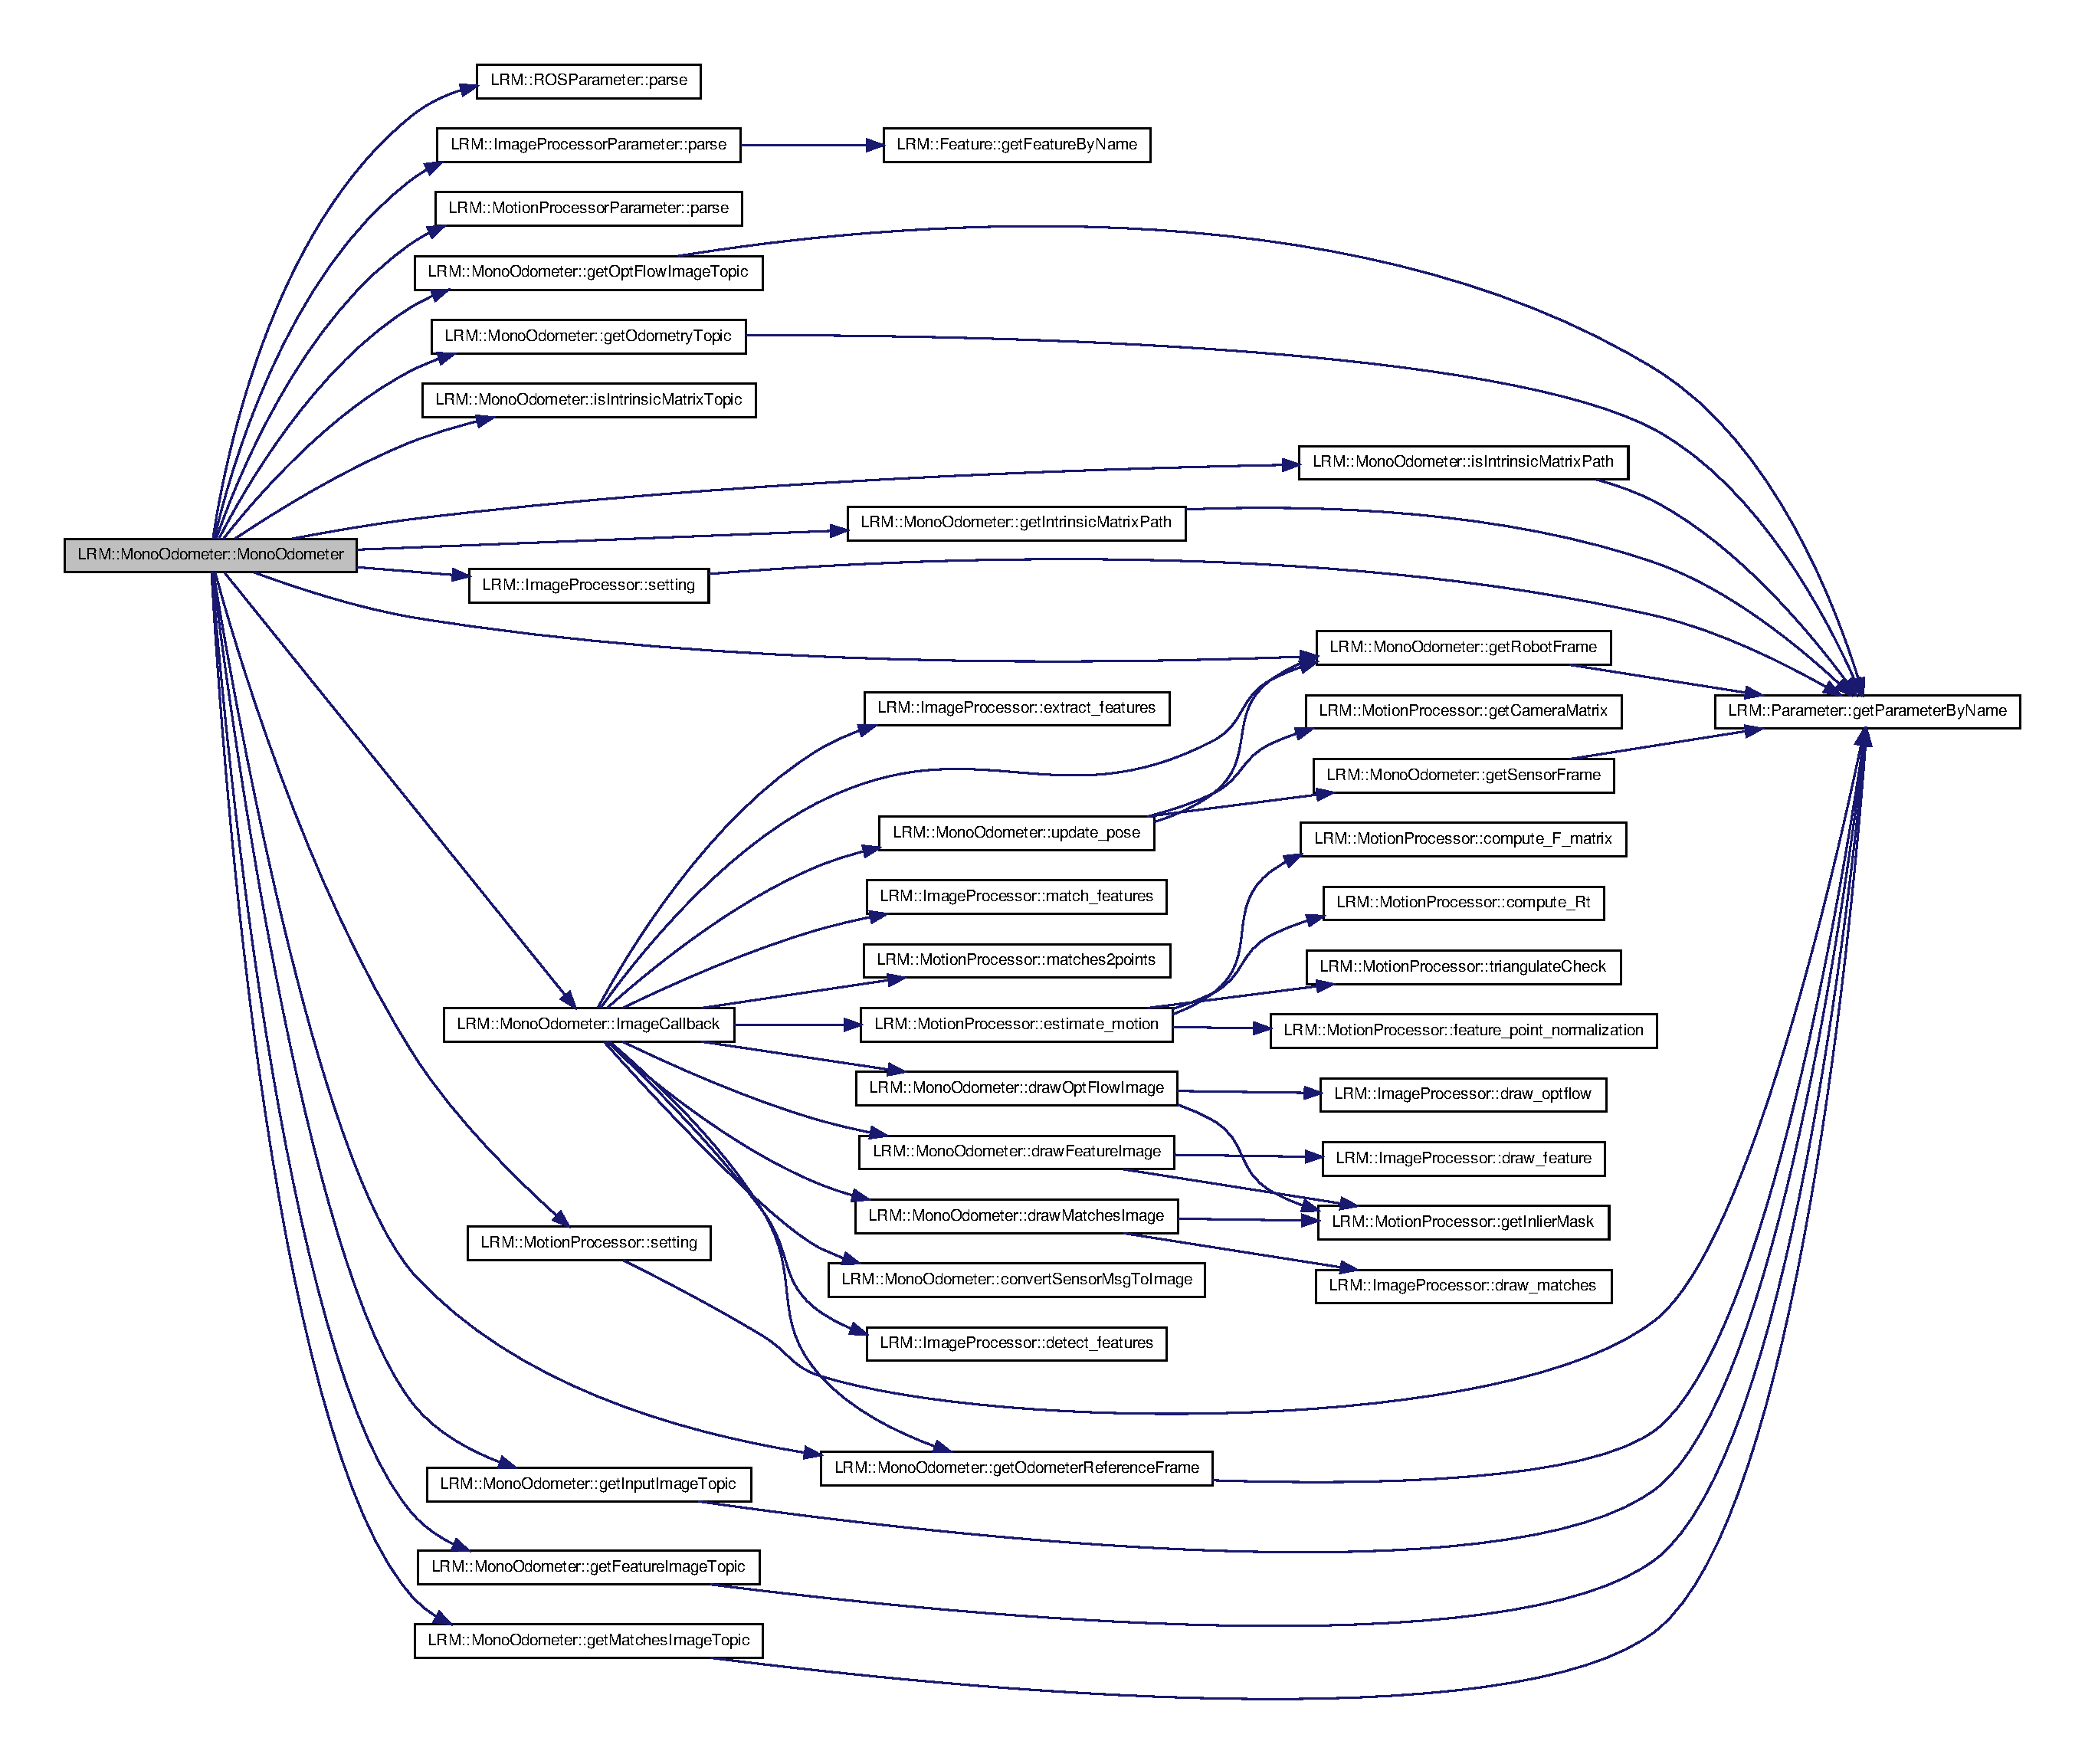
\includegraphics[width=350pt]{classLRM_1_1MonoOdometer_ae849abdcd3e0b49be6b1672b292c86ba_cgraph}
\end{center}
\end{figure}


\hypertarget{classLRM_1_1MonoOdometer_aadca97effbd3970022f8fdfa42c1177b}{\index{\-L\-R\-M\-::\-Mono\-Odometer@{\-L\-R\-M\-::\-Mono\-Odometer}!$\sim$\-Mono\-Odometer@{$\sim$\-Mono\-Odometer}}
\index{$\sim$\-Mono\-Odometer@{$\sim$\-Mono\-Odometer}!LRM::MonoOdometer@{\-L\-R\-M\-::\-Mono\-Odometer}}
\subsubsection[{$\sim$\-Mono\-Odometer}]{\setlength{\rightskip}{0pt plus 5cm}{\bf \-L\-R\-M\-::\-Mono\-Odometer\-::$\sim$\-Mono\-Odometer} (
\begin{DoxyParamCaption}
{}
\end{DoxyParamCaption}
)}}\label{classLRM_1_1MonoOdometer_aadca97effbd3970022f8fdfa42c1177b}


\subsection{\-Member \-Function \-Documentation}
\hypertarget{classLRM_1_1MonoOdometer_ab33c598738d4c565cae80ca110f3ab63}{\index{\-L\-R\-M\-::\-Mono\-Odometer@{\-L\-R\-M\-::\-Mono\-Odometer}!convert\-Sensor\-Msg\-To\-Image@{convert\-Sensor\-Msg\-To\-Image}}
\index{convert\-Sensor\-Msg\-To\-Image@{convert\-Sensor\-Msg\-To\-Image}!LRM::MonoOdometer@{\-L\-R\-M\-::\-Mono\-Odometer}}
\subsubsection[{convert\-Sensor\-Msg\-To\-Image}]{\setlength{\rightskip}{0pt plus 5cm}int {\bf \-L\-R\-M\-::\-Mono\-Odometer\-::convert\-Sensor\-Msg\-To\-Image} (
\begin{DoxyParamCaption}
\item[{const sensor\-\_\-msgs\-::\-Image\-Const\-Ptr \&}]{msg, }
\item[{cv\-\_\-bridge\-::\-Cv\-Image\-Const\-Ptr \&}]{image}
\end{DoxyParamCaption}
)\hspace{0.3cm}{\ttfamily  \mbox{[}private\mbox{]}}}}\label{classLRM_1_1MonoOdometer_ab33c598738d4c565cae80ca110f3ab63}


\-Converts a sensor message to a grayscale image. 


\begin{DoxyParams}{\-Parameters}
{\em msg} & \-Sensor image \\
\hline
{\em image} & \-Output image \\
\hline
\end{DoxyParams}
\begin{DoxyReturn}{\-Returns}
\-Error code 
\end{DoxyReturn}
\hypertarget{classLRM_1_1MonoOdometer_acdfde454162a9fba808c5e99069e5831}{\index{\-L\-R\-M\-::\-Mono\-Odometer@{\-L\-R\-M\-::\-Mono\-Odometer}!draw\-Feature\-Image@{draw\-Feature\-Image}}
\index{draw\-Feature\-Image@{draw\-Feature\-Image}!LRM::MonoOdometer@{\-L\-R\-M\-::\-Mono\-Odometer}}
\subsubsection[{draw\-Feature\-Image}]{\setlength{\rightskip}{0pt plus 5cm}int {\bf \-L\-R\-M\-::\-Mono\-Odometer\-::draw\-Feature\-Image} (
\begin{DoxyParamCaption}
{}
\end{DoxyParamCaption}
)\hspace{0.3cm}{\ttfamily  \mbox{[}private\mbox{]}}}}\label{classLRM_1_1MonoOdometer_acdfde454162a9fba808c5e99069e5831}


\-Here is the call graph for this function\-:\nopagebreak
\begin{figure}[H]
\begin{center}
\leavevmode
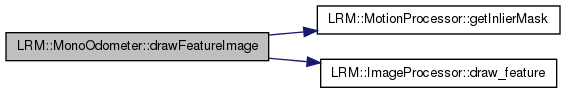
\includegraphics[width=350pt]{classLRM_1_1MonoOdometer_acdfde454162a9fba808c5e99069e5831_cgraph}
\end{center}
\end{figure}


\hypertarget{classLRM_1_1MonoOdometer_a0e648fa164c12e1bb405c5e0de9607cf}{\index{\-L\-R\-M\-::\-Mono\-Odometer@{\-L\-R\-M\-::\-Mono\-Odometer}!draw\-Matches\-Image@{draw\-Matches\-Image}}
\index{draw\-Matches\-Image@{draw\-Matches\-Image}!LRM::MonoOdometer@{\-L\-R\-M\-::\-Mono\-Odometer}}
\subsubsection[{draw\-Matches\-Image}]{\setlength{\rightskip}{0pt plus 5cm}int {\bf \-L\-R\-M\-::\-Mono\-Odometer\-::draw\-Matches\-Image} (
\begin{DoxyParamCaption}
{}
\end{DoxyParamCaption}
)\hspace{0.3cm}{\ttfamily  \mbox{[}private\mbox{]}}}}\label{classLRM_1_1MonoOdometer_a0e648fa164c12e1bb405c5e0de9607cf}


\-Here is the call graph for this function\-:\nopagebreak
\begin{figure}[H]
\begin{center}
\leavevmode
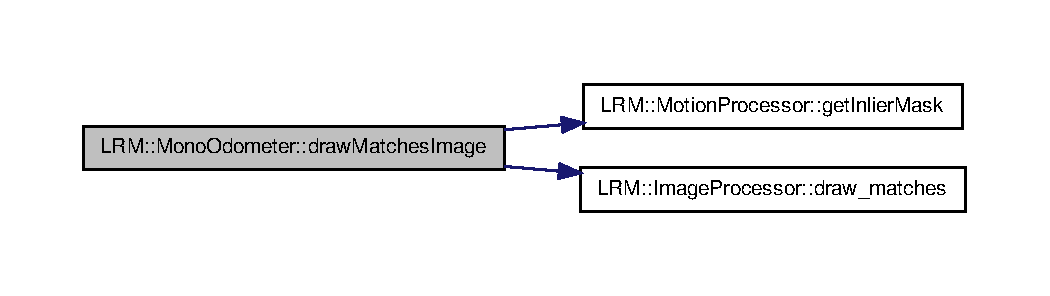
\includegraphics[width=350pt]{classLRM_1_1MonoOdometer_a0e648fa164c12e1bb405c5e0de9607cf_cgraph}
\end{center}
\end{figure}


\hypertarget{classLRM_1_1MonoOdometer_ac3e11ffd664dfd8b06068f77dd475ed4}{\index{\-L\-R\-M\-::\-Mono\-Odometer@{\-L\-R\-M\-::\-Mono\-Odometer}!draw\-Opt\-Flow\-Image@{draw\-Opt\-Flow\-Image}}
\index{draw\-Opt\-Flow\-Image@{draw\-Opt\-Flow\-Image}!LRM::MonoOdometer@{\-L\-R\-M\-::\-Mono\-Odometer}}
\subsubsection[{draw\-Opt\-Flow\-Image}]{\setlength{\rightskip}{0pt plus 5cm}int {\bf \-L\-R\-M\-::\-Mono\-Odometer\-::draw\-Opt\-Flow\-Image} (
\begin{DoxyParamCaption}
{}
\end{DoxyParamCaption}
)\hspace{0.3cm}{\ttfamily  \mbox{[}private\mbox{]}}}}\label{classLRM_1_1MonoOdometer_ac3e11ffd664dfd8b06068f77dd475ed4}


\-Here is the call graph for this function\-:\nopagebreak
\begin{figure}[H]
\begin{center}
\leavevmode
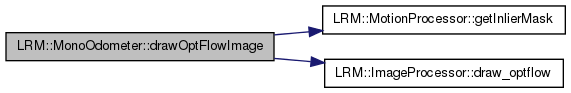
\includegraphics[width=350pt]{classLRM_1_1MonoOdometer_ac3e11ffd664dfd8b06068f77dd475ed4_cgraph}
\end{center}
\end{figure}


\hypertarget{classLRM_1_1MonoOdometer_a68f5f4b33141cd2a2ea92db6197db65c}{\index{\-L\-R\-M\-::\-Mono\-Odometer@{\-L\-R\-M\-::\-Mono\-Odometer}!get\-Feature\-Image\-Topic@{get\-Feature\-Image\-Topic}}
\index{get\-Feature\-Image\-Topic@{get\-Feature\-Image\-Topic}!LRM::MonoOdometer@{\-L\-R\-M\-::\-Mono\-Odometer}}
\subsubsection[{get\-Feature\-Image\-Topic}]{\setlength{\rightskip}{0pt plus 5cm}std\-::string {\bf \-L\-R\-M\-::\-Mono\-Odometer\-::get\-Feature\-Image\-Topic} (
\begin{DoxyParamCaption}
{}
\end{DoxyParamCaption}
)\hspace{0.3cm}{\ttfamily  \mbox{[}inline\mbox{]}}}}\label{classLRM_1_1MonoOdometer_a68f5f4b33141cd2a2ea92db6197db65c}


\-Here is the call graph for this function\-:\nopagebreak
\begin{figure}[H]
\begin{center}
\leavevmode
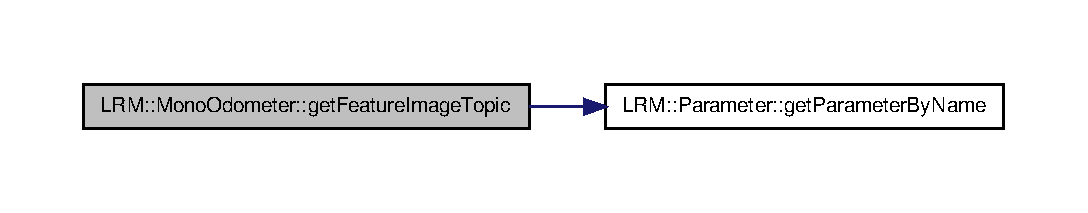
\includegraphics[width=350pt]{classLRM_1_1MonoOdometer_a68f5f4b33141cd2a2ea92db6197db65c_cgraph}
\end{center}
\end{figure}


\hypertarget{classLRM_1_1MonoOdometer_a3174620fdca5f375ec38bc0709c2e1e0}{\index{\-L\-R\-M\-::\-Mono\-Odometer@{\-L\-R\-M\-::\-Mono\-Odometer}!get\-Input\-Image\-Topic@{get\-Input\-Image\-Topic}}
\index{get\-Input\-Image\-Topic@{get\-Input\-Image\-Topic}!LRM::MonoOdometer@{\-L\-R\-M\-::\-Mono\-Odometer}}
\subsubsection[{get\-Input\-Image\-Topic}]{\setlength{\rightskip}{0pt plus 5cm}std\-::string {\bf \-L\-R\-M\-::\-Mono\-Odometer\-::get\-Input\-Image\-Topic} (
\begin{DoxyParamCaption}
{}
\end{DoxyParamCaption}
)\hspace{0.3cm}{\ttfamily  \mbox{[}inline\mbox{]}}}}\label{classLRM_1_1MonoOdometer_a3174620fdca5f375ec38bc0709c2e1e0}


\-Here is the call graph for this function\-:\nopagebreak
\begin{figure}[H]
\begin{center}
\leavevmode
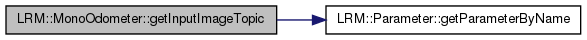
\includegraphics[width=350pt]{classLRM_1_1MonoOdometer_a3174620fdca5f375ec38bc0709c2e1e0_cgraph}
\end{center}
\end{figure}


\hypertarget{classLRM_1_1MonoOdometer_ab75736159a13ba537ed8615c84853243}{\index{\-L\-R\-M\-::\-Mono\-Odometer@{\-L\-R\-M\-::\-Mono\-Odometer}!get\-Intrinsic\-Matrix\-Path@{get\-Intrinsic\-Matrix\-Path}}
\index{get\-Intrinsic\-Matrix\-Path@{get\-Intrinsic\-Matrix\-Path}!LRM::MonoOdometer@{\-L\-R\-M\-::\-Mono\-Odometer}}
\subsubsection[{get\-Intrinsic\-Matrix\-Path}]{\setlength{\rightskip}{0pt plus 5cm}std\-::string {\bf \-L\-R\-M\-::\-Mono\-Odometer\-::get\-Intrinsic\-Matrix\-Path} (
\begin{DoxyParamCaption}
{}
\end{DoxyParamCaption}
)\hspace{0.3cm}{\ttfamily  \mbox{[}inline\mbox{]}}}}\label{classLRM_1_1MonoOdometer_ab75736159a13ba537ed8615c84853243}


\-Here is the call graph for this function\-:\nopagebreak
\begin{figure}[H]
\begin{center}
\leavevmode
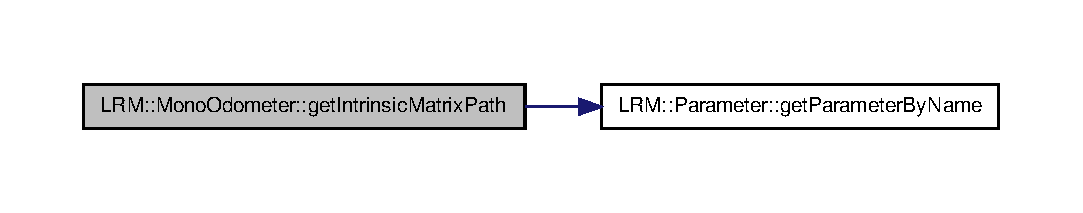
\includegraphics[width=350pt]{classLRM_1_1MonoOdometer_ab75736159a13ba537ed8615c84853243_cgraph}
\end{center}
\end{figure}


\hypertarget{classLRM_1_1MonoOdometer_a0b5b603776c1c011d1268dc029dee6ae}{\index{\-L\-R\-M\-::\-Mono\-Odometer@{\-L\-R\-M\-::\-Mono\-Odometer}!get\-Matches\-Image\-Topic@{get\-Matches\-Image\-Topic}}
\index{get\-Matches\-Image\-Topic@{get\-Matches\-Image\-Topic}!LRM::MonoOdometer@{\-L\-R\-M\-::\-Mono\-Odometer}}
\subsubsection[{get\-Matches\-Image\-Topic}]{\setlength{\rightskip}{0pt plus 5cm}std\-::string {\bf \-L\-R\-M\-::\-Mono\-Odometer\-::get\-Matches\-Image\-Topic} (
\begin{DoxyParamCaption}
{}
\end{DoxyParamCaption}
)\hspace{0.3cm}{\ttfamily  \mbox{[}inline\mbox{]}}}}\label{classLRM_1_1MonoOdometer_a0b5b603776c1c011d1268dc029dee6ae}


\-Here is the call graph for this function\-:\nopagebreak
\begin{figure}[H]
\begin{center}
\leavevmode
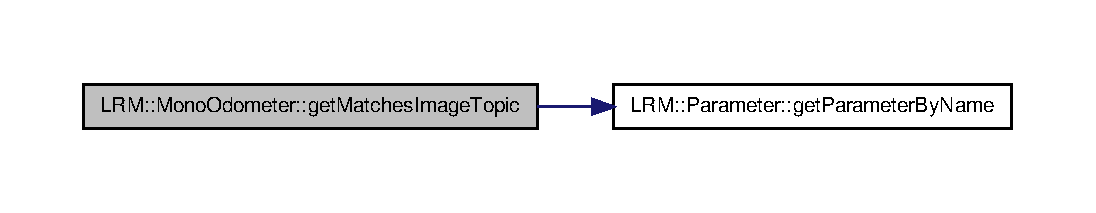
\includegraphics[width=350pt]{classLRM_1_1MonoOdometer_a0b5b603776c1c011d1268dc029dee6ae_cgraph}
\end{center}
\end{figure}


\hypertarget{classLRM_1_1MonoOdometer_ac989d0a61c0b18c7e538732668953fa1}{\index{\-L\-R\-M\-::\-Mono\-Odometer@{\-L\-R\-M\-::\-Mono\-Odometer}!get\-Odometer\-Reference\-Frame@{get\-Odometer\-Reference\-Frame}}
\index{get\-Odometer\-Reference\-Frame@{get\-Odometer\-Reference\-Frame}!LRM::MonoOdometer@{\-L\-R\-M\-::\-Mono\-Odometer}}
\subsubsection[{get\-Odometer\-Reference\-Frame}]{\setlength{\rightskip}{0pt plus 5cm}std\-::string {\bf \-L\-R\-M\-::\-Mono\-Odometer\-::get\-Odometer\-Reference\-Frame} (
\begin{DoxyParamCaption}
{}
\end{DoxyParamCaption}
)\hspace{0.3cm}{\ttfamily  \mbox{[}inline\mbox{]}}}}\label{classLRM_1_1MonoOdometer_ac989d0a61c0b18c7e538732668953fa1}


\-Here is the call graph for this function\-:\nopagebreak
\begin{figure}[H]
\begin{center}
\leavevmode
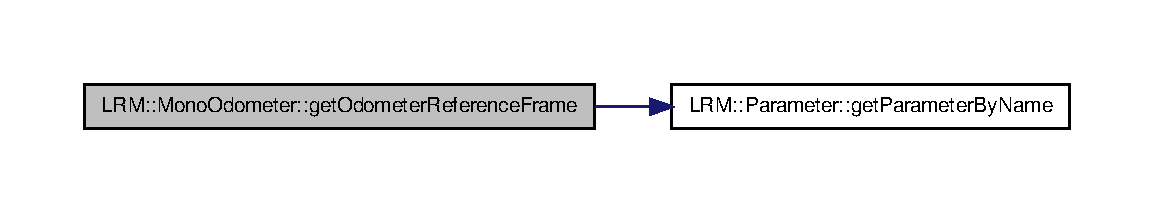
\includegraphics[width=350pt]{classLRM_1_1MonoOdometer_ac989d0a61c0b18c7e538732668953fa1_cgraph}
\end{center}
\end{figure}


\hypertarget{classLRM_1_1MonoOdometer_a16eaa3716cb077ef993fa66a582fe65e}{\index{\-L\-R\-M\-::\-Mono\-Odometer@{\-L\-R\-M\-::\-Mono\-Odometer}!get\-Odometry\-Topic@{get\-Odometry\-Topic}}
\index{get\-Odometry\-Topic@{get\-Odometry\-Topic}!LRM::MonoOdometer@{\-L\-R\-M\-::\-Mono\-Odometer}}
\subsubsection[{get\-Odometry\-Topic}]{\setlength{\rightskip}{0pt plus 5cm}std\-::string {\bf \-L\-R\-M\-::\-Mono\-Odometer\-::get\-Odometry\-Topic} (
\begin{DoxyParamCaption}
{}
\end{DoxyParamCaption}
)\hspace{0.3cm}{\ttfamily  \mbox{[}inline\mbox{]}}}}\label{classLRM_1_1MonoOdometer_a16eaa3716cb077ef993fa66a582fe65e}


\-Here is the call graph for this function\-:\nopagebreak
\begin{figure}[H]
\begin{center}
\leavevmode
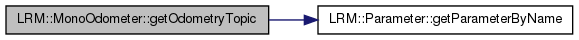
\includegraphics[width=350pt]{classLRM_1_1MonoOdometer_a16eaa3716cb077ef993fa66a582fe65e_cgraph}
\end{center}
\end{figure}


\hypertarget{classLRM_1_1MonoOdometer_acde0fd05b19f524bace7c71de9a0cc36}{\index{\-L\-R\-M\-::\-Mono\-Odometer@{\-L\-R\-M\-::\-Mono\-Odometer}!get\-Opt\-Flow\-Image\-Topic@{get\-Opt\-Flow\-Image\-Topic}}
\index{get\-Opt\-Flow\-Image\-Topic@{get\-Opt\-Flow\-Image\-Topic}!LRM::MonoOdometer@{\-L\-R\-M\-::\-Mono\-Odometer}}
\subsubsection[{get\-Opt\-Flow\-Image\-Topic}]{\setlength{\rightskip}{0pt plus 5cm}std\-::string {\bf \-L\-R\-M\-::\-Mono\-Odometer\-::get\-Opt\-Flow\-Image\-Topic} (
\begin{DoxyParamCaption}
{}
\end{DoxyParamCaption}
)\hspace{0.3cm}{\ttfamily  \mbox{[}inline\mbox{]}}}}\label{classLRM_1_1MonoOdometer_acde0fd05b19f524bace7c71de9a0cc36}


\-Here is the call graph for this function\-:\nopagebreak
\begin{figure}[H]
\begin{center}
\leavevmode
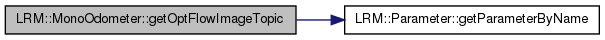
\includegraphics[width=350pt]{classLRM_1_1MonoOdometer_acde0fd05b19f524bace7c71de9a0cc36_cgraph}
\end{center}
\end{figure}


\hypertarget{classLRM_1_1MonoOdometer_a3550a896dd2e212fa177d7401f1a5b61}{\index{\-L\-R\-M\-::\-Mono\-Odometer@{\-L\-R\-M\-::\-Mono\-Odometer}!get\-Robot\-Frame@{get\-Robot\-Frame}}
\index{get\-Robot\-Frame@{get\-Robot\-Frame}!LRM::MonoOdometer@{\-L\-R\-M\-::\-Mono\-Odometer}}
\subsubsection[{get\-Robot\-Frame}]{\setlength{\rightskip}{0pt plus 5cm}std\-::string {\bf \-L\-R\-M\-::\-Mono\-Odometer\-::get\-Robot\-Frame} (
\begin{DoxyParamCaption}
{}
\end{DoxyParamCaption}
)\hspace{0.3cm}{\ttfamily  \mbox{[}inline\mbox{]}}}}\label{classLRM_1_1MonoOdometer_a3550a896dd2e212fa177d7401f1a5b61}


\-Here is the call graph for this function\-:\nopagebreak
\begin{figure}[H]
\begin{center}
\leavevmode
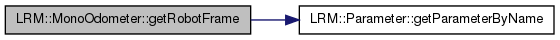
\includegraphics[width=350pt]{classLRM_1_1MonoOdometer_a3550a896dd2e212fa177d7401f1a5b61_cgraph}
\end{center}
\end{figure}


\hypertarget{classLRM_1_1MonoOdometer_a72b47de741d2c273a34c7d4e9a093092}{\index{\-L\-R\-M\-::\-Mono\-Odometer@{\-L\-R\-M\-::\-Mono\-Odometer}!get\-Sensor\-Frame@{get\-Sensor\-Frame}}
\index{get\-Sensor\-Frame@{get\-Sensor\-Frame}!LRM::MonoOdometer@{\-L\-R\-M\-::\-Mono\-Odometer}}
\subsubsection[{get\-Sensor\-Frame}]{\setlength{\rightskip}{0pt plus 5cm}std\-::string {\bf \-L\-R\-M\-::\-Mono\-Odometer\-::get\-Sensor\-Frame} (
\begin{DoxyParamCaption}
{}
\end{DoxyParamCaption}
)\hspace{0.3cm}{\ttfamily  \mbox{[}inline\mbox{]}}}}\label{classLRM_1_1MonoOdometer_a72b47de741d2c273a34c7d4e9a093092}


\-Here is the call graph for this function\-:\nopagebreak
\begin{figure}[H]
\begin{center}
\leavevmode
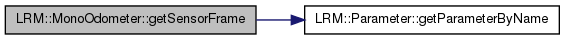
\includegraphics[width=350pt]{classLRM_1_1MonoOdometer_a72b47de741d2c273a34c7d4e9a093092_cgraph}
\end{center}
\end{figure}


\hypertarget{classLRM_1_1MonoOdometer_a7205e77893b1f9d4c37de616519ef5ed}{\index{\-L\-R\-M\-::\-Mono\-Odometer@{\-L\-R\-M\-::\-Mono\-Odometer}!\-Image\-Callback@{\-Image\-Callback}}
\index{\-Image\-Callback@{\-Image\-Callback}!LRM::MonoOdometer@{\-L\-R\-M\-::\-Mono\-Odometer}}
\subsubsection[{\-Image\-Callback}]{\setlength{\rightskip}{0pt plus 5cm}void {\bf \-L\-R\-M\-::\-Mono\-Odometer\-::\-Image\-Callback} (
\begin{DoxyParamCaption}
\item[{const sensor\-\_\-msgs\-::\-Image\-Const\-Ptr \&}]{msg}
\end{DoxyParamCaption}
)}}\label{classLRM_1_1MonoOdometer_a7205e77893b1f9d4c37de616519ef5ed}


\-The \-Image \-Callback method is responsible for handling the income messages from the camera device and extract the frame features and descriptors. 


\begin{DoxyParams}[1]{\-Parameters}
\mbox{\tt in}  & {\em msg} & \-Income message from the defined camera topic. \\
\hline
\end{DoxyParams}
\begin{DoxyRefDesc}{\-Todo}
\item[\hyperlink{todo__todo000001}{\-Todo}]\-What happens when it's not possible to estimate a motion? \-Kalman? \end{DoxyRefDesc}


\-Here is the call graph for this function\-:\nopagebreak
\begin{figure}[H]
\begin{center}
\leavevmode
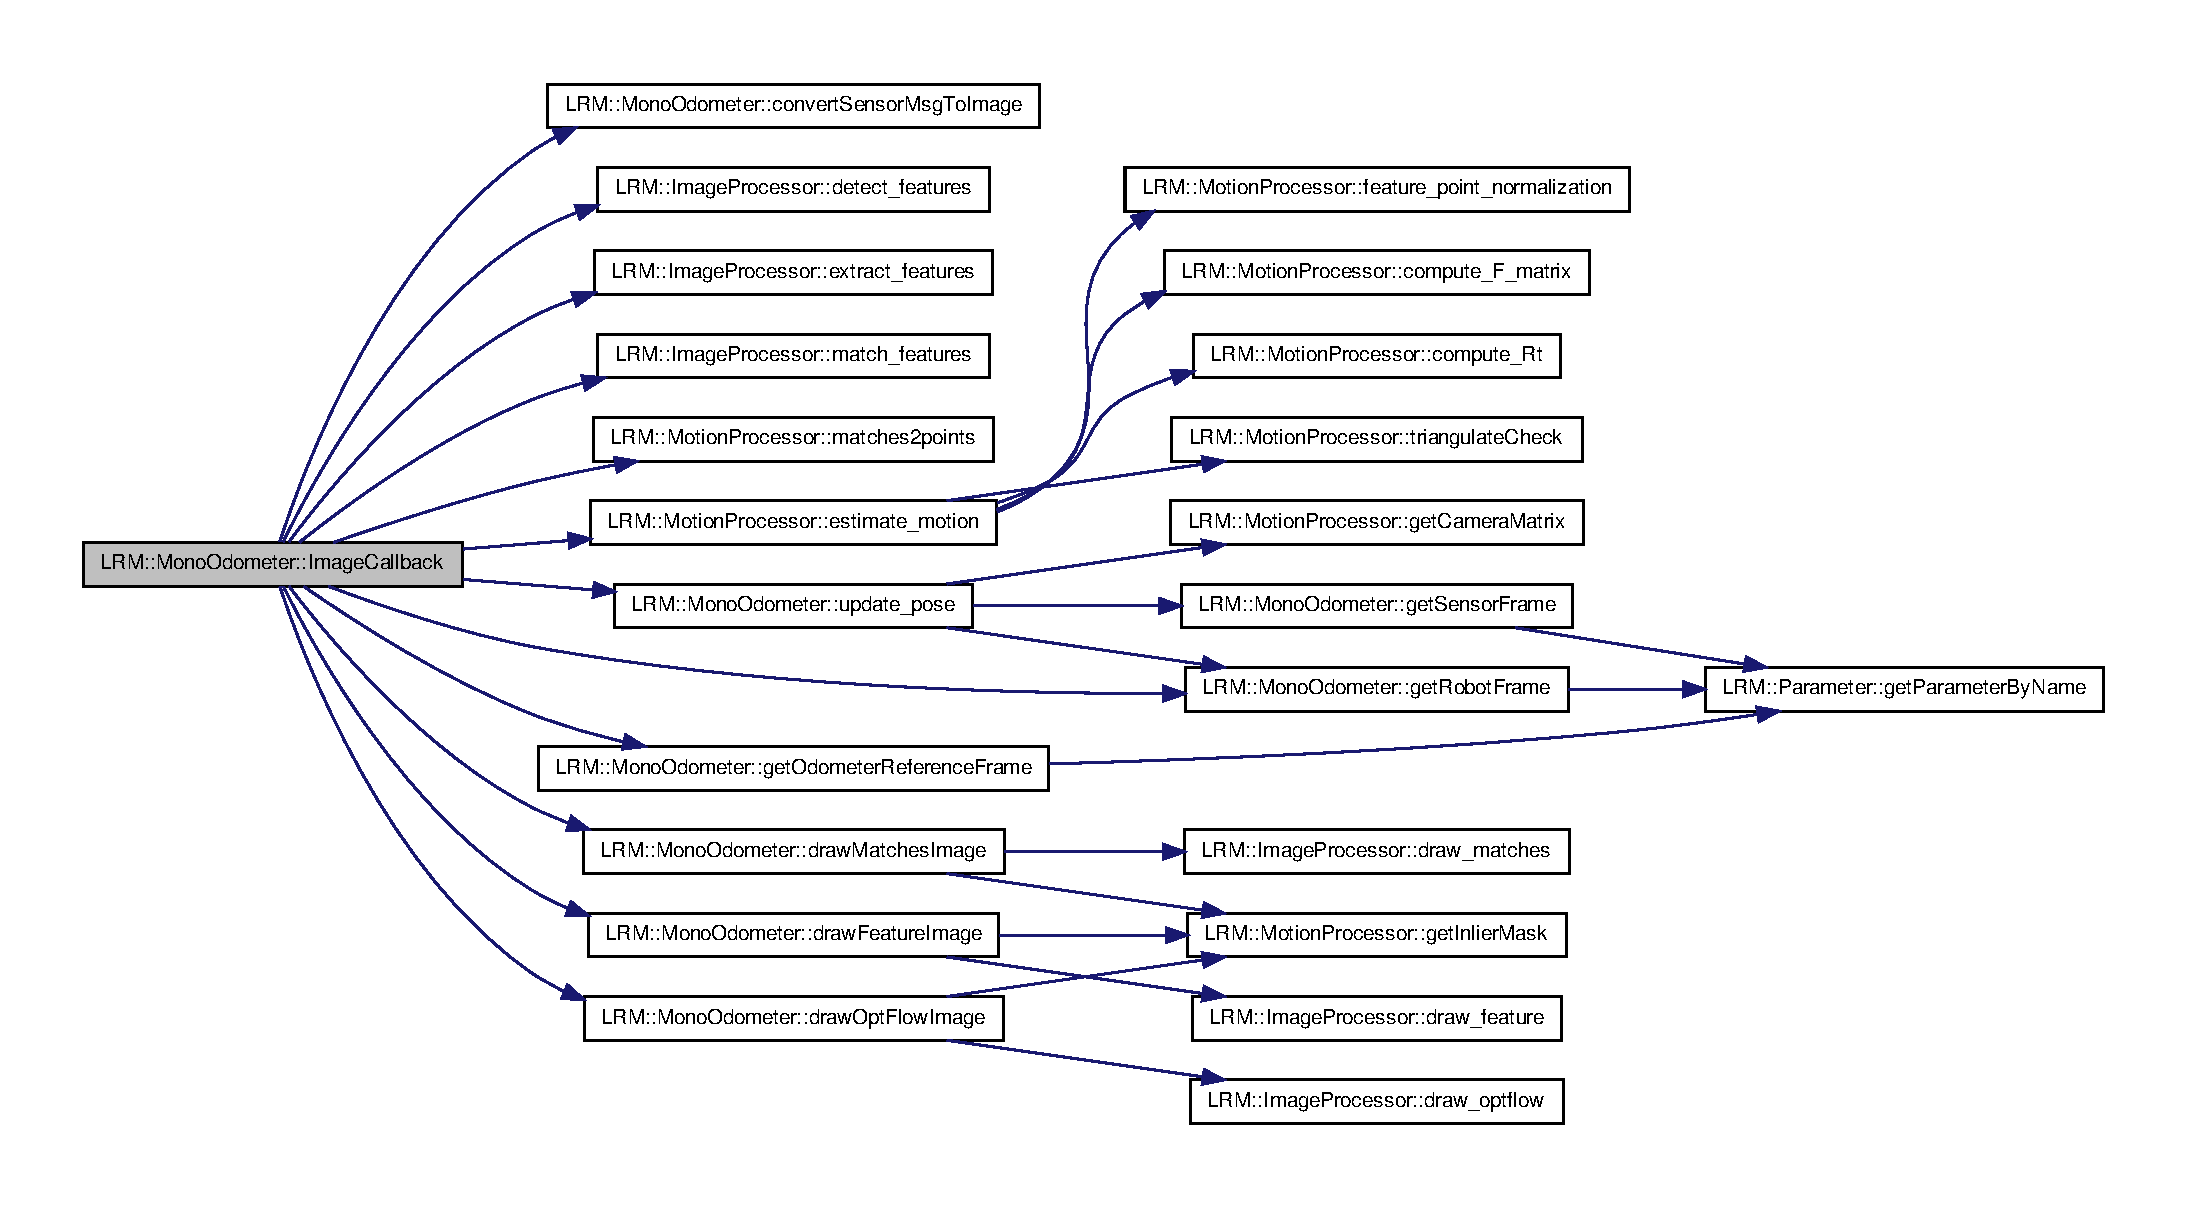
\includegraphics[width=350pt]{classLRM_1_1MonoOdometer_a7205e77893b1f9d4c37de616519ef5ed_cgraph}
\end{center}
\end{figure}


\hypertarget{classLRM_1_1MonoOdometer_aaea86d0c2fc1119b066b310451be4a67}{\index{\-L\-R\-M\-::\-Mono\-Odometer@{\-L\-R\-M\-::\-Mono\-Odometer}!is\-Intrinsic\-Matrix\-Path@{is\-Intrinsic\-Matrix\-Path}}
\index{is\-Intrinsic\-Matrix\-Path@{is\-Intrinsic\-Matrix\-Path}!LRM::MonoOdometer@{\-L\-R\-M\-::\-Mono\-Odometer}}
\subsubsection[{is\-Intrinsic\-Matrix\-Path}]{\setlength{\rightskip}{0pt plus 5cm}bool {\bf \-L\-R\-M\-::\-Mono\-Odometer\-::is\-Intrinsic\-Matrix\-Path} (
\begin{DoxyParamCaption}
{}
\end{DoxyParamCaption}
)\hspace{0.3cm}{\ttfamily  \mbox{[}inline\mbox{]}}}}\label{classLRM_1_1MonoOdometer_aaea86d0c2fc1119b066b310451be4a67}


\-Here is the call graph for this function\-:\nopagebreak
\begin{figure}[H]
\begin{center}
\leavevmode
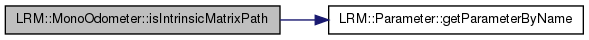
\includegraphics[width=350pt]{classLRM_1_1MonoOdometer_aaea86d0c2fc1119b066b310451be4a67_cgraph}
\end{center}
\end{figure}


\hypertarget{classLRM_1_1MonoOdometer_a8c7914efde9c07323c171d7adfaf656e}{\index{\-L\-R\-M\-::\-Mono\-Odometer@{\-L\-R\-M\-::\-Mono\-Odometer}!update\-\_\-pose@{update\-\_\-pose}}
\index{update\-\_\-pose@{update\-\_\-pose}!LRM::MonoOdometer@{\-L\-R\-M\-::\-Mono\-Odometer}}
\subsubsection[{update\-\_\-pose}]{\setlength{\rightskip}{0pt plus 5cm}int {\bf \-L\-R\-M\-::\-Mono\-Odometer\-::update\-\_\-pose} (
\begin{DoxyParamCaption}
{}
\end{DoxyParamCaption}
)\hspace{0.3cm}{\ttfamily  \mbox{[}private\mbox{]}}}}\label{classLRM_1_1MonoOdometer_a8c7914efde9c07323c171d7adfaf656e}


\-Here is the call graph for this function\-:\nopagebreak
\begin{figure}[H]
\begin{center}
\leavevmode
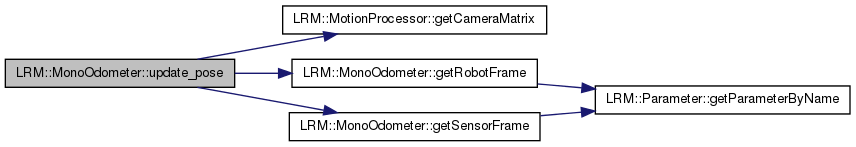
\includegraphics[width=350pt]{classLRM_1_1MonoOdometer_a8c7914efde9c07323c171d7adfaf656e_cgraph}
\end{center}
\end{figure}




\subsection{\-Member \-Data \-Documentation}
\hypertarget{classLRM_1_1MonoOdometer_a311831c9328491cde059e17706fd9bdc}{\index{\-L\-R\-M\-::\-Mono\-Odometer@{\-L\-R\-M\-::\-Mono\-Odometer}!base\-\_\-to\-\_\-sensor@{base\-\_\-to\-\_\-sensor}}
\index{base\-\_\-to\-\_\-sensor@{base\-\_\-to\-\_\-sensor}!LRM::MonoOdometer@{\-L\-R\-M\-::\-Mono\-Odometer}}
\subsubsection[{base\-\_\-to\-\_\-sensor}]{\setlength{\rightskip}{0pt plus 5cm}tf\-::\-Stamped\-Transform {\bf \-L\-R\-M\-::\-Mono\-Odometer\-::base\-\_\-to\-\_\-sensor}\hspace{0.3cm}{\ttfamily  \mbox{[}private\mbox{]}}}}\label{classLRM_1_1MonoOdometer_a311831c9328491cde059e17706fd9bdc}
\hypertarget{classLRM_1_1MonoOdometer_a166844b373399a94d688234592ae8468}{\index{\-L\-R\-M\-::\-Mono\-Odometer@{\-L\-R\-M\-::\-Mono\-Odometer}!feature\-\_\-image@{feature\-\_\-image}}
\index{feature\-\_\-image@{feature\-\_\-image}!LRM::MonoOdometer@{\-L\-R\-M\-::\-Mono\-Odometer}}
\subsubsection[{feature\-\_\-image}]{\setlength{\rightskip}{0pt plus 5cm}cv\-\_\-bridge\-::\-Cv\-Image {\bf \-L\-R\-M\-::\-Mono\-Odometer\-::feature\-\_\-image}\hspace{0.3cm}{\ttfamily  \mbox{[}private\mbox{]}}}}\label{classLRM_1_1MonoOdometer_a166844b373399a94d688234592ae8468}
\hypertarget{classLRM_1_1MonoOdometer_a49bef96a5413beea489f87dbb16eaf70}{\index{\-L\-R\-M\-::\-Mono\-Odometer@{\-L\-R\-M\-::\-Mono\-Odometer}!img\-\_\-proc@{img\-\_\-proc}}
\index{img\-\_\-proc@{img\-\_\-proc}!LRM::MonoOdometer@{\-L\-R\-M\-::\-Mono\-Odometer}}
\subsubsection[{img\-\_\-proc}]{\setlength{\rightskip}{0pt plus 5cm}{\bf \-Image\-Processor} {\bf \-L\-R\-M\-::\-Mono\-Odometer\-::img\-\_\-proc}\hspace{0.3cm}{\ttfamily  \mbox{[}private\mbox{]}}}}\label{classLRM_1_1MonoOdometer_a49bef96a5413beea489f87dbb16eaf70}
\hypertarget{classLRM_1_1MonoOdometer_a1bf24a1abdef05b79b54813058cad4a7}{\index{\-L\-R\-M\-::\-Mono\-Odometer@{\-L\-R\-M\-::\-Mono\-Odometer}!img\-\_\-proc\-\_\-parameter@{img\-\_\-proc\-\_\-parameter}}
\index{img\-\_\-proc\-\_\-parameter@{img\-\_\-proc\-\_\-parameter}!LRM::MonoOdometer@{\-L\-R\-M\-::\-Mono\-Odometer}}
\subsubsection[{img\-\_\-proc\-\_\-parameter}]{\setlength{\rightskip}{0pt plus 5cm}{\bf \-Image\-Processor\-Parameter} {\bf \-L\-R\-M\-::\-Mono\-Odometer\-::img\-\_\-proc\-\_\-parameter}\hspace{0.3cm}{\ttfamily  \mbox{[}private\mbox{]}}}}\label{classLRM_1_1MonoOdometer_a1bf24a1abdef05b79b54813058cad4a7}
\hypertarget{classLRM_1_1MonoOdometer_ad191c12993c8e8ee9200f71aec07057c}{\index{\-L\-R\-M\-::\-Mono\-Odometer@{\-L\-R\-M\-::\-Mono\-Odometer}!input\-\_\-image\-\_\-subscriber@{input\-\_\-image\-\_\-subscriber}}
\index{input\-\_\-image\-\_\-subscriber@{input\-\_\-image\-\_\-subscriber}!LRM::MonoOdometer@{\-L\-R\-M\-::\-Mono\-Odometer}}
\subsubsection[{input\-\_\-image\-\_\-subscriber}]{\setlength{\rightskip}{0pt plus 5cm}image\-\_\-transport\-::\-Subscriber {\bf \-L\-R\-M\-::\-Mono\-Odometer\-::input\-\_\-image\-\_\-subscriber}\hspace{0.3cm}{\ttfamily  \mbox{[}private\mbox{]}}}}\label{classLRM_1_1MonoOdometer_ad191c12993c8e8ee9200f71aec07057c}
\hypertarget{classLRM_1_1MonoOdometer_a7f874bb9b174d7a38085782377d5f195}{\index{\-L\-R\-M\-::\-Mono\-Odometer@{\-L\-R\-M\-::\-Mono\-Odometer}!\-K@{\-K}}
\index{\-K@{\-K}!LRM::MonoOdometer@{\-L\-R\-M\-::\-Mono\-Odometer}}
\subsubsection[{\-K}]{\setlength{\rightskip}{0pt plus 5cm}cv\-::\-Mat {\bf \-L\-R\-M\-::\-Mono\-Odometer\-::\-K}\hspace{0.3cm}{\ttfamily  \mbox{[}private\mbox{]}}}}\label{classLRM_1_1MonoOdometer_a7f874bb9b174d7a38085782377d5f195}
\hypertarget{classLRM_1_1MonoOdometer_aefc5720615c86208707622253d2e08ed}{\index{\-L\-R\-M\-::\-Mono\-Odometer@{\-L\-R\-M\-::\-Mono\-Odometer}!matches@{matches}}
\index{matches@{matches}!LRM::MonoOdometer@{\-L\-R\-M\-::\-Mono\-Odometer}}
\subsubsection[{matches}]{\setlength{\rightskip}{0pt plus 5cm}std\-::vector$<$cv\-::\-D\-Match$>$ {\bf \-L\-R\-M\-::\-Mono\-Odometer\-::matches}\hspace{0.3cm}{\ttfamily  \mbox{[}private\mbox{]}}}}\label{classLRM_1_1MonoOdometer_aefc5720615c86208707622253d2e08ed}
\hypertarget{classLRM_1_1MonoOdometer_a1646743b51e5e0386def055e0265aaf2}{\index{\-L\-R\-M\-::\-Mono\-Odometer@{\-L\-R\-M\-::\-Mono\-Odometer}!matches\-\_\-image@{matches\-\_\-image}}
\index{matches\-\_\-image@{matches\-\_\-image}!LRM::MonoOdometer@{\-L\-R\-M\-::\-Mono\-Odometer}}
\subsubsection[{matches\-\_\-image}]{\setlength{\rightskip}{0pt plus 5cm}cv\-\_\-bridge\-::\-Cv\-Image {\bf \-L\-R\-M\-::\-Mono\-Odometer\-::matches\-\_\-image}\hspace{0.3cm}{\ttfamily  \mbox{[}private\mbox{]}}}}\label{classLRM_1_1MonoOdometer_a1646743b51e5e0386def055e0265aaf2}
\hypertarget{classLRM_1_1MonoOdometer_a91b2fd9ac3051a11e7008c2e3740a382}{\index{\-L\-R\-M\-::\-Mono\-Odometer@{\-L\-R\-M\-::\-Mono\-Odometer}!mot\-\_\-proc@{mot\-\_\-proc}}
\index{mot\-\_\-proc@{mot\-\_\-proc}!LRM::MonoOdometer@{\-L\-R\-M\-::\-Mono\-Odometer}}
\subsubsection[{mot\-\_\-proc}]{\setlength{\rightskip}{0pt plus 5cm}{\bf \-Motion\-Processor} {\bf \-L\-R\-M\-::\-Mono\-Odometer\-::mot\-\_\-proc}\hspace{0.3cm}{\ttfamily  \mbox{[}private\mbox{]}}}}\label{classLRM_1_1MonoOdometer_a91b2fd9ac3051a11e7008c2e3740a382}
\hypertarget{classLRM_1_1MonoOdometer_a8bf0ca69100b032fe3c73fb1e0bed318}{\index{\-L\-R\-M\-::\-Mono\-Odometer@{\-L\-R\-M\-::\-Mono\-Odometer}!mot\-\_\-proc\-\_\-parameter@{mot\-\_\-proc\-\_\-parameter}}
\index{mot\-\_\-proc\-\_\-parameter@{mot\-\_\-proc\-\_\-parameter}!LRM::MonoOdometer@{\-L\-R\-M\-::\-Mono\-Odometer}}
\subsubsection[{mot\-\_\-proc\-\_\-parameter}]{\setlength{\rightskip}{0pt plus 5cm}{\bf \-Motion\-Processor\-Parameter} {\bf \-L\-R\-M\-::\-Mono\-Odometer\-::mot\-\_\-proc\-\_\-parameter}\hspace{0.3cm}{\ttfamily  \mbox{[}private\mbox{]}}}}\label{classLRM_1_1MonoOdometer_a8bf0ca69100b032fe3c73fb1e0bed318}
\hypertarget{classLRM_1_1MonoOdometer_a85bf06a46a0367a821f145e1c3f51e8c}{\index{\-L\-R\-M\-::\-Mono\-Odometer@{\-L\-R\-M\-::\-Mono\-Odometer}!odom\-\_\-broadcaster@{odom\-\_\-broadcaster}}
\index{odom\-\_\-broadcaster@{odom\-\_\-broadcaster}!LRM::MonoOdometer@{\-L\-R\-M\-::\-Mono\-Odometer}}
\subsubsection[{odom\-\_\-broadcaster}]{\setlength{\rightskip}{0pt plus 5cm}tf\-::\-Transform\-Broadcaster {\bf \-L\-R\-M\-::\-Mono\-Odometer\-::odom\-\_\-broadcaster}\hspace{0.3cm}{\ttfamily  \mbox{[}private\mbox{]}}}}\label{classLRM_1_1MonoOdometer_a85bf06a46a0367a821f145e1c3f51e8c}
\hypertarget{classLRM_1_1MonoOdometer_afdc33ed78a3234b3469e094b23b4d511}{\index{\-L\-R\-M\-::\-Mono\-Odometer@{\-L\-R\-M\-::\-Mono\-Odometer}!odometry@{odometry}}
\index{odometry@{odometry}!LRM::MonoOdometer@{\-L\-R\-M\-::\-Mono\-Odometer}}
\subsubsection[{odometry}]{\setlength{\rightskip}{0pt plus 5cm}nav\-\_\-msgs\-::\-Odometry {\bf \-L\-R\-M\-::\-Mono\-Odometer\-::odometry}\hspace{0.3cm}{\ttfamily  \mbox{[}private\mbox{]}}}}\label{classLRM_1_1MonoOdometer_afdc33ed78a3234b3469e094b23b4d511}
\hypertarget{classLRM_1_1MonoOdometer_a113a9a4905bb7c9f19df55610802ffec}{\index{\-L\-R\-M\-::\-Mono\-Odometer@{\-L\-R\-M\-::\-Mono\-Odometer}!odometry\-\_\-advertiser@{odometry\-\_\-advertiser}}
\index{odometry\-\_\-advertiser@{odometry\-\_\-advertiser}!LRM::MonoOdometer@{\-L\-R\-M\-::\-Mono\-Odometer}}
\subsubsection[{odometry\-\_\-advertiser}]{\setlength{\rightskip}{0pt plus 5cm}ros\-::\-Publisher {\bf \-L\-R\-M\-::\-Mono\-Odometer\-::odometry\-\_\-advertiser}\hspace{0.3cm}{\ttfamily  \mbox{[}private\mbox{]}}}}\label{classLRM_1_1MonoOdometer_a113a9a4905bb7c9f19df55610802ffec}
\hypertarget{classLRM_1_1MonoOdometer_a5f9b4ef57cf2b7d88bb92c8269a8792d}{\index{\-L\-R\-M\-::\-Mono\-Odometer@{\-L\-R\-M\-::\-Mono\-Odometer}!optflow\-\_\-image@{optflow\-\_\-image}}
\index{optflow\-\_\-image@{optflow\-\_\-image}!LRM::MonoOdometer@{\-L\-R\-M\-::\-Mono\-Odometer}}
\subsubsection[{optflow\-\_\-image}]{\setlength{\rightskip}{0pt plus 5cm}cv\-\_\-bridge\-::\-Cv\-Image {\bf \-L\-R\-M\-::\-Mono\-Odometer\-::optflow\-\_\-image}\hspace{0.3cm}{\ttfamily  \mbox{[}private\mbox{]}}}}\label{classLRM_1_1MonoOdometer_a5f9b4ef57cf2b7d88bb92c8269a8792d}
\hypertarget{classLRM_1_1MonoOdometer_abcc8b0e66d3629d66b74e8d857adea9e}{\index{\-L\-R\-M\-::\-Mono\-Odometer@{\-L\-R\-M\-::\-Mono\-Odometer}!output\-\_\-feature\-\_\-advertiser@{output\-\_\-feature\-\_\-advertiser}}
\index{output\-\_\-feature\-\_\-advertiser@{output\-\_\-feature\-\_\-advertiser}!LRM::MonoOdometer@{\-L\-R\-M\-::\-Mono\-Odometer}}
\subsubsection[{output\-\_\-feature\-\_\-advertiser}]{\setlength{\rightskip}{0pt plus 5cm}image\-\_\-transport\-::\-Publisher {\bf \-L\-R\-M\-::\-Mono\-Odometer\-::output\-\_\-feature\-\_\-advertiser}\hspace{0.3cm}{\ttfamily  \mbox{[}private\mbox{]}}}}\label{classLRM_1_1MonoOdometer_abcc8b0e66d3629d66b74e8d857adea9e}
\hypertarget{classLRM_1_1MonoOdometer_ab3e372106292ea873dc5428e1b3d0026}{\index{\-L\-R\-M\-::\-Mono\-Odometer@{\-L\-R\-M\-::\-Mono\-Odometer}!output\-\_\-matches\-\_\-advertiser@{output\-\_\-matches\-\_\-advertiser}}
\index{output\-\_\-matches\-\_\-advertiser@{output\-\_\-matches\-\_\-advertiser}!LRM::MonoOdometer@{\-L\-R\-M\-::\-Mono\-Odometer}}
\subsubsection[{output\-\_\-matches\-\_\-advertiser}]{\setlength{\rightskip}{0pt plus 5cm}image\-\_\-transport\-::\-Publisher {\bf \-L\-R\-M\-::\-Mono\-Odometer\-::output\-\_\-matches\-\_\-advertiser}\hspace{0.3cm}{\ttfamily  \mbox{[}private\mbox{]}}}}\label{classLRM_1_1MonoOdometer_ab3e372106292ea873dc5428e1b3d0026}
\hypertarget{classLRM_1_1MonoOdometer_a2f9dcb6ceed7b4b85e0df512fc297105}{\index{\-L\-R\-M\-::\-Mono\-Odometer@{\-L\-R\-M\-::\-Mono\-Odometer}!output\-\_\-optflow\-\_\-advertiser@{output\-\_\-optflow\-\_\-advertiser}}
\index{output\-\_\-optflow\-\_\-advertiser@{output\-\_\-optflow\-\_\-advertiser}!LRM::MonoOdometer@{\-L\-R\-M\-::\-Mono\-Odometer}}
\subsubsection[{output\-\_\-optflow\-\_\-advertiser}]{\setlength{\rightskip}{0pt plus 5cm}image\-\_\-transport\-::\-Publisher {\bf \-L\-R\-M\-::\-Mono\-Odometer\-::output\-\_\-optflow\-\_\-advertiser}\hspace{0.3cm}{\ttfamily  \mbox{[}private\mbox{]}}}}\label{classLRM_1_1MonoOdometer_a2f9dcb6ceed7b4b85e0df512fc297105}
\hypertarget{classLRM_1_1MonoOdometer_a086c208e839df4586e99d417c60a3d77}{\index{\-L\-R\-M\-::\-Mono\-Odometer@{\-L\-R\-M\-::\-Mono\-Odometer}!pose@{pose}}
\index{pose@{pose}!LRM::MonoOdometer@{\-L\-R\-M\-::\-Mono\-Odometer}}
\subsubsection[{pose}]{\setlength{\rightskip}{0pt plus 5cm}tf\-::\-Transform {\bf \-L\-R\-M\-::\-Mono\-Odometer\-::pose}\hspace{0.3cm}{\ttfamily  \mbox{[}private\mbox{]}}}}\label{classLRM_1_1MonoOdometer_a086c208e839df4586e99d417c60a3d77}
\hypertarget{classLRM_1_1MonoOdometer_a7bf26df30d6cebf7e6c5b85c2318ff51}{\index{\-L\-R\-M\-::\-Mono\-Odometer@{\-L\-R\-M\-::\-Mono\-Odometer}!query\-\_\-desc@{query\-\_\-desc}}
\index{query\-\_\-desc@{query\-\_\-desc}!LRM::MonoOdometer@{\-L\-R\-M\-::\-Mono\-Odometer}}
\subsubsection[{query\-\_\-desc}]{\setlength{\rightskip}{0pt plus 5cm}cv\-::\-Mat {\bf \-L\-R\-M\-::\-Mono\-Odometer\-::query\-\_\-desc}\hspace{0.3cm}{\ttfamily  \mbox{[}private\mbox{]}}}}\label{classLRM_1_1MonoOdometer_a7bf26df30d6cebf7e6c5b85c2318ff51}
\hypertarget{classLRM_1_1MonoOdometer_a1fbec0b090c10b1c542bd86f18795a14}{\index{\-L\-R\-M\-::\-Mono\-Odometer@{\-L\-R\-M\-::\-Mono\-Odometer}!query\-\_\-image@{query\-\_\-image}}
\index{query\-\_\-image@{query\-\_\-image}!LRM::MonoOdometer@{\-L\-R\-M\-::\-Mono\-Odometer}}
\subsubsection[{query\-\_\-image}]{\setlength{\rightskip}{0pt plus 5cm}cv\-\_\-bridge\-::\-Cv\-Image\-Const\-Ptr {\bf \-L\-R\-M\-::\-Mono\-Odometer\-::query\-\_\-image}\hspace{0.3cm}{\ttfamily  \mbox{[}private\mbox{]}}}}\label{classLRM_1_1MonoOdometer_a1fbec0b090c10b1c542bd86f18795a14}


\-Current image. 

\hypertarget{classLRM_1_1MonoOdometer_a18d64f992353bf50e1421a1cb9ca32f2}{\index{\-L\-R\-M\-::\-Mono\-Odometer@{\-L\-R\-M\-::\-Mono\-Odometer}!query\-\_\-kpts@{query\-\_\-kpts}}
\index{query\-\_\-kpts@{query\-\_\-kpts}!LRM::MonoOdometer@{\-L\-R\-M\-::\-Mono\-Odometer}}
\subsubsection[{query\-\_\-kpts}]{\setlength{\rightskip}{0pt plus 5cm}std\-::vector$<$cv\-::\-Key\-Point$>$ {\bf \-L\-R\-M\-::\-Mono\-Odometer\-::query\-\_\-kpts}\hspace{0.3cm}{\ttfamily  \mbox{[}private\mbox{]}}}}\label{classLRM_1_1MonoOdometer_a18d64f992353bf50e1421a1cb9ca32f2}


\-Current image keypoints. 

\hypertarget{classLRM_1_1MonoOdometer_a4d269a8b3827580e73515e8f958e2283}{\index{\-L\-R\-M\-::\-Mono\-Odometer@{\-L\-R\-M\-::\-Mono\-Odometer}!query\-\_\-pts@{query\-\_\-pts}}
\index{query\-\_\-pts@{query\-\_\-pts}!LRM::MonoOdometer@{\-L\-R\-M\-::\-Mono\-Odometer}}
\subsubsection[{query\-\_\-pts}]{\setlength{\rightskip}{0pt plus 5cm}std\-::vector$<$cv\-::\-Point2d$>$ {\bf \-L\-R\-M\-::\-Mono\-Odometer\-::query\-\_\-pts}\hspace{0.3cm}{\ttfamily  \mbox{[}private\mbox{]}}}}\label{classLRM_1_1MonoOdometer_a4d269a8b3827580e73515e8f958e2283}
\hypertarget{classLRM_1_1MonoOdometer_ae201ba1988badf708c046e1b29b70ab1}{\index{\-L\-R\-M\-::\-Mono\-Odometer@{\-L\-R\-M\-::\-Mono\-Odometer}!query\-\_\-timestamp@{query\-\_\-timestamp}}
\index{query\-\_\-timestamp@{query\-\_\-timestamp}!LRM::MonoOdometer@{\-L\-R\-M\-::\-Mono\-Odometer}}
\subsubsection[{query\-\_\-timestamp}]{\setlength{\rightskip}{0pt plus 5cm}ros\-::\-Time {\bf \-L\-R\-M\-::\-Mono\-Odometer\-::query\-\_\-timestamp}\hspace{0.3cm}{\ttfamily  \mbox{[}private\mbox{]}}}}\label{classLRM_1_1MonoOdometer_ae201ba1988badf708c046e1b29b70ab1}
\hypertarget{classLRM_1_1MonoOdometer_a7667abb4e8d035e25811c63e6af42ae3}{\index{\-L\-R\-M\-::\-Mono\-Odometer@{\-L\-R\-M\-::\-Mono\-Odometer}!ros\-\_\-parameter@{ros\-\_\-parameter}}
\index{ros\-\_\-parameter@{ros\-\_\-parameter}!LRM::MonoOdometer@{\-L\-R\-M\-::\-Mono\-Odometer}}
\subsubsection[{ros\-\_\-parameter}]{\setlength{\rightskip}{0pt plus 5cm}{\bf \-R\-O\-S\-Parameter} {\bf \-L\-R\-M\-::\-Mono\-Odometer\-::ros\-\_\-parameter}\hspace{0.3cm}{\ttfamily  \mbox{[}private\mbox{]}}}}\label{classLRM_1_1MonoOdometer_a7667abb4e8d035e25811c63e6af42ae3}
\hypertarget{classLRM_1_1MonoOdometer_aa17423bfec7b2a995672d40cc6ed4fbe}{\index{\-L\-R\-M\-::\-Mono\-Odometer@{\-L\-R\-M\-::\-Mono\-Odometer}!tf\-\_\-listener@{tf\-\_\-listener}}
\index{tf\-\_\-listener@{tf\-\_\-listener}!LRM::MonoOdometer@{\-L\-R\-M\-::\-Mono\-Odometer}}
\subsubsection[{tf\-\_\-listener}]{\setlength{\rightskip}{0pt plus 5cm}tf\-::\-Transform\-Listener {\bf \-L\-R\-M\-::\-Mono\-Odometer\-::tf\-\_\-listener}\hspace{0.3cm}{\ttfamily  \mbox{[}private\mbox{]}}}}\label{classLRM_1_1MonoOdometer_aa17423bfec7b2a995672d40cc6ed4fbe}
\hypertarget{classLRM_1_1MonoOdometer_aae6c2096b1b0c785548bc57cf6557427}{\index{\-L\-R\-M\-::\-Mono\-Odometer@{\-L\-R\-M\-::\-Mono\-Odometer}!train\-\_\-desc@{train\-\_\-desc}}
\index{train\-\_\-desc@{train\-\_\-desc}!LRM::MonoOdometer@{\-L\-R\-M\-::\-Mono\-Odometer}}
\subsubsection[{train\-\_\-desc}]{\setlength{\rightskip}{0pt plus 5cm}cv\-::\-Mat {\bf \-L\-R\-M\-::\-Mono\-Odometer\-::train\-\_\-desc}\hspace{0.3cm}{\ttfamily  \mbox{[}private\mbox{]}}}}\label{classLRM_1_1MonoOdometer_aae6c2096b1b0c785548bc57cf6557427}
\hypertarget{classLRM_1_1MonoOdometer_a91ee6e52006559ba0f769a2ccc06fa64}{\index{\-L\-R\-M\-::\-Mono\-Odometer@{\-L\-R\-M\-::\-Mono\-Odometer}!train\-\_\-image@{train\-\_\-image}}
\index{train\-\_\-image@{train\-\_\-image}!LRM::MonoOdometer@{\-L\-R\-M\-::\-Mono\-Odometer}}
\subsubsection[{train\-\_\-image}]{\setlength{\rightskip}{0pt plus 5cm}cv\-\_\-bridge\-::\-Cv\-Image\-Const\-Ptr {\bf \-L\-R\-M\-::\-Mono\-Odometer\-::train\-\_\-image}\hspace{0.3cm}{\ttfamily  \mbox{[}private\mbox{]}}}}\label{classLRM_1_1MonoOdometer_a91ee6e52006559ba0f769a2ccc06fa64}


\-Previous image. 

\hypertarget{classLRM_1_1MonoOdometer_a98515916ee97beaefb9bbcf07cd02d1b}{\index{\-L\-R\-M\-::\-Mono\-Odometer@{\-L\-R\-M\-::\-Mono\-Odometer}!train\-\_\-kpts@{train\-\_\-kpts}}
\index{train\-\_\-kpts@{train\-\_\-kpts}!LRM::MonoOdometer@{\-L\-R\-M\-::\-Mono\-Odometer}}
\subsubsection[{train\-\_\-kpts}]{\setlength{\rightskip}{0pt plus 5cm}std\-::vector$<$cv\-::\-Key\-Point$>$ {\bf \-L\-R\-M\-::\-Mono\-Odometer\-::train\-\_\-kpts}\hspace{0.3cm}{\ttfamily  \mbox{[}private\mbox{]}}}}\label{classLRM_1_1MonoOdometer_a98515916ee97beaefb9bbcf07cd02d1b}


\-Previous image keypoints. 

\hypertarget{classLRM_1_1MonoOdometer_accbdc3f32cf2fb8e75f3f40cd8a4e60e}{\index{\-L\-R\-M\-::\-Mono\-Odometer@{\-L\-R\-M\-::\-Mono\-Odometer}!train\-\_\-pts@{train\-\_\-pts}}
\index{train\-\_\-pts@{train\-\_\-pts}!LRM::MonoOdometer@{\-L\-R\-M\-::\-Mono\-Odometer}}
\subsubsection[{train\-\_\-pts}]{\setlength{\rightskip}{0pt plus 5cm}std\-::vector$<$cv\-::\-Point2d$>$ {\bf \-L\-R\-M\-::\-Mono\-Odometer\-::train\-\_\-pts}\hspace{0.3cm}{\ttfamily  \mbox{[}private\mbox{]}}}}\label{classLRM_1_1MonoOdometer_accbdc3f32cf2fb8e75f3f40cd8a4e60e}
\hypertarget{classLRM_1_1MonoOdometer_a7024b12b516c41771d59046471ea7319}{\index{\-L\-R\-M\-::\-Mono\-Odometer@{\-L\-R\-M\-::\-Mono\-Odometer}!train\-\_\-timestamp@{train\-\_\-timestamp}}
\index{train\-\_\-timestamp@{train\-\_\-timestamp}!LRM::MonoOdometer@{\-L\-R\-M\-::\-Mono\-Odometer}}
\subsubsection[{train\-\_\-timestamp}]{\setlength{\rightskip}{0pt plus 5cm}ros\-::\-Time {\bf \-L\-R\-M\-::\-Mono\-Odometer\-::train\-\_\-timestamp}\hspace{0.3cm}{\ttfamily  \mbox{[}private\mbox{]}}}}\label{classLRM_1_1MonoOdometer_a7024b12b516c41771d59046471ea7319}


\-The documentation for this class was generated from the following files\-:\begin{DoxyCompactItemize}
\item 
include/\hyperlink{mono__odometer_8h}{mono\-\_\-odometer.\-h}\item 
src/\hyperlink{mono__odometer_8cpp}{mono\-\_\-odometer.\-cpp}\end{DoxyCompactItemize}

\hypertarget{classLRM_1_1Motion}{\section{\-L\-R\-M\-:\-:\-Motion \-Class \-Reference}
\label{classLRM_1_1Motion}\index{\-L\-R\-M\-::\-Motion@{\-L\-R\-M\-::\-Motion}}
}


{\ttfamily \#include $<$motion.\-h$>$}

\subsection*{\-Public \-Member \-Functions}
\begin{DoxyCompactItemize}
\item 
\hyperlink{classLRM_1_1Motion_a42e6da69a192faa122baca4c4a3e558a}{\-Motion} ()
\item 
virtual \hyperlink{classLRM_1_1Motion_a8a1247f6604ff86e083e59e37662c26d}{$\sim$\-Motion} ()
\end{DoxyCompactItemize}


\subsection{\-Constructor \& \-Destructor \-Documentation}
\hypertarget{classLRM_1_1Motion_a42e6da69a192faa122baca4c4a3e558a}{\index{\-L\-R\-M\-::\-Motion@{\-L\-R\-M\-::\-Motion}!\-Motion@{\-Motion}}
\index{\-Motion@{\-Motion}!LRM::Motion@{\-L\-R\-M\-::\-Motion}}
\subsubsection[{\-Motion}]{\setlength{\rightskip}{0pt plus 5cm}{\bf \-L\-R\-M\-::\-Motion\-::\-Motion} (
\begin{DoxyParamCaption}
{}
\end{DoxyParamCaption}
)}}\label{classLRM_1_1Motion_a42e6da69a192faa122baca4c4a3e558a}
\hypertarget{classLRM_1_1Motion_a8a1247f6604ff86e083e59e37662c26d}{\index{\-L\-R\-M\-::\-Motion@{\-L\-R\-M\-::\-Motion}!$\sim$\-Motion@{$\sim$\-Motion}}
\index{$\sim$\-Motion@{$\sim$\-Motion}!LRM::Motion@{\-L\-R\-M\-::\-Motion}}
\subsubsection[{$\sim$\-Motion}]{\setlength{\rightskip}{0pt plus 5cm}{\bf \-L\-R\-M\-::\-Motion\-::$\sim$\-Motion} (
\begin{DoxyParamCaption}
{}
\end{DoxyParamCaption}
)\hspace{0.3cm}{\ttfamily  \mbox{[}virtual\mbox{]}}}}\label{classLRM_1_1Motion_a8a1247f6604ff86e083e59e37662c26d}


\-The documentation for this class was generated from the following files\-:\begin{DoxyCompactItemize}
\item 
include/\hyperlink{motion_8h}{motion.\-h}\item 
src/\hyperlink{motion_8cpp}{motion.\-cpp}\end{DoxyCompactItemize}

\chapter{\-File \-Documentation}
\hypertarget{feature_8h}{\section{include/feature.h \-File \-Reference}
\label{feature_8h}\index{include/feature.\-h@{include/feature.\-h}}
}
{\ttfamily \#include $<$vector$>$}\*
{\ttfamily \#include $<$boost/smart\-\_\-ptr.\-hpp$>$}\*
{\ttfamily \#include $<$opencv2/imgproc/imgproc.\-hpp$>$}\*
\-Include dependency graph for feature.\-h\-:\nopagebreak
\begin{figure}[H]
\begin{center}
\leavevmode
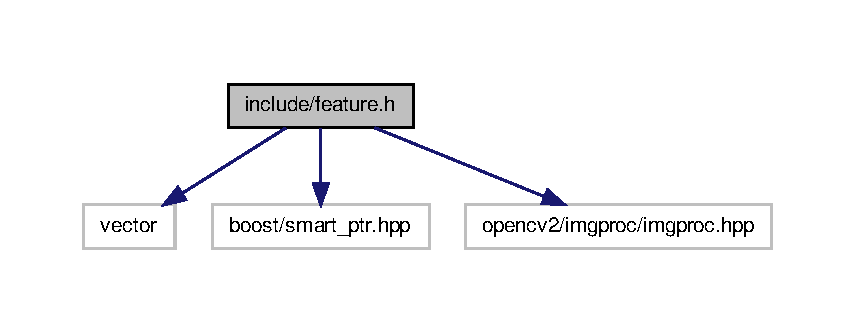
\includegraphics[width=350pt]{feature_8h__incl}
\end{center}
\end{figure}
\-This graph shows which files directly or indirectly include this file\-:\nopagebreak
\begin{figure}[H]
\begin{center}
\leavevmode
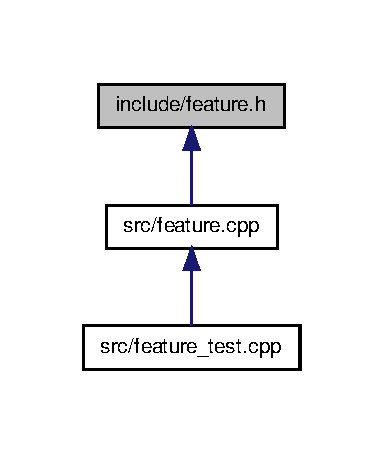
\includegraphics[width=184pt]{feature_8h__dep__incl}
\end{center}
\end{figure}
\subsection*{\-Classes}
\begin{DoxyCompactItemize}
\item 
class \hyperlink{classLRM_1_1Feature}{\-L\-R\-M\-::\-Feature}
\item 
class \hyperlink{classLRM_1_1Descriptor}{\-L\-R\-M\-::\-Descriptor}
\end{DoxyCompactItemize}
\subsection*{\-Namespaces}
\begin{DoxyCompactItemize}
\item 
namespace \hyperlink{namespaceLRM}{\-L\-R\-M}
\end{DoxyCompactItemize}

\hypertarget{frame_8h}{\section{include/frame.h \-File \-Reference}
\label{frame_8h}\index{include/frame.\-h@{include/frame.\-h}}
}
{\ttfamily \#include $<$ros/ros.\-h$>$}\*
{\ttfamily \#include $<$vector$>$}\*
\-Include dependency graph for frame.\-h\-:
\nopagebreak
\begin{figure}[H]
\begin{center}
\leavevmode
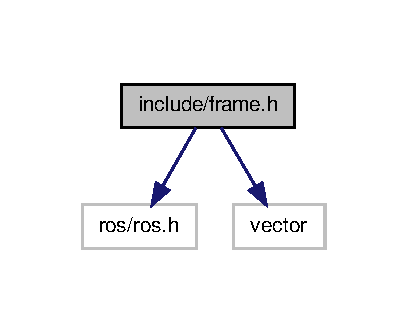
\includegraphics[width=196pt]{frame_8h__incl}
\end{center}
\end{figure}
\-This graph shows which files directly or indirectly include this file\-:\nopagebreak
\begin{figure}[H]
\begin{center}
\leavevmode
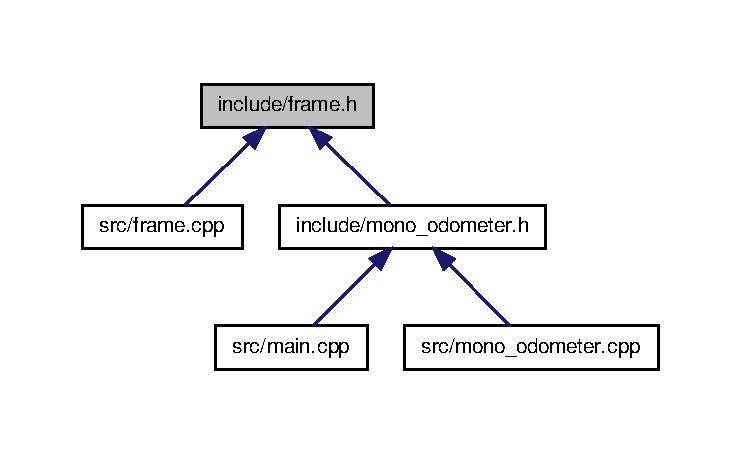
\includegraphics[width=350pt]{frame_8h__dep__incl}
\end{center}
\end{figure}
\subsection*{\-Classes}
\begin{DoxyCompactItemize}
\item 
class \hyperlink{classLRM_1_1Frame}{\-L\-R\-M\-::\-Frame}
\end{DoxyCompactItemize}
\subsection*{\-Namespaces}
\begin{DoxyCompactItemize}
\item 
namespace \hyperlink{namespaceLRM}{\-L\-R\-M}
\end{DoxyCompactItemize}
\subsection*{\-Typedefs}
\begin{DoxyCompactItemize}
\item 
typedef cv\-::\-Point2f \hyperlink{namespaceLRM_a83d84534368107ba7cdbde260cfc3070}{\-L\-R\-M\-::\-Feature}
\item 
typedef cv\-::\-Rect \hyperlink{namespaceLRM_aa94fd446417fb568723141ba14bde953}{\-L\-R\-M\-::\-Descriptor}
\end{DoxyCompactItemize}
\subsection*{\-Enumerations}
\begin{DoxyCompactItemize}
\item 
enum \hyperlink{namespaceLRM_a8eb6956b84fb7d27bce5af771937794f}{\-L\-R\-M\-::feature\-\_\-t} \{ \hyperlink{namespaceLRM_a8eb6956b84fb7d27bce5af771937794fa8e3a2d26370c85d7adb97cbbd40abc72}{\-L\-R\-M\-::\-S\-H\-I\-\_\-\-T\-O\-M\-A\-S\-I}, 
\hyperlink{namespaceLRM_a8eb6956b84fb7d27bce5af771937794fa82f8a835c4a989b4beddacd8082dc75d}{\-L\-R\-M\-::\-H\-A\-R\-R\-I\-S}
 \}
\begin{DoxyCompactList}\small\item\em \-Types of possible features. \end{DoxyCompactList}\item 
enum \hyperlink{namespaceLRM_ad31d475a7f32e1bd208beb34aabc6fa9}{\-L\-R\-M\-::descriptor\-\_\-t} \{ \hyperlink{namespaceLRM_ad31d475a7f32e1bd208beb34aabc6fa9a1e43a18048d2fc5fc782f2eebce0d585}{\-L\-R\-M\-::\-S\-S\-D}
 \}
\begin{DoxyCompactList}\small\item\em \-Types of possible descriptors. \end{DoxyCompactList}\end{DoxyCompactItemize}

\hypertarget{mono__odometer_8h}{\section{include/mono\-\_\-odometer.h \-File \-Reference}
\label{mono__odometer_8h}\index{include/mono\-\_\-odometer.\-h@{include/mono\-\_\-odometer.\-h}}
}
{\ttfamily \#include \char`\"{}core.\-h\char`\"{}}\*
{\ttfamily \#include \char`\"{}parameter.\-h\char`\"{}}\*
{\ttfamily \#include \char`\"{}image\-\_\-processor.\-h\char`\"{}}\*
{\ttfamily \#include \char`\"{}motion\-\_\-processor.\-h\char`\"{}}\*
{\ttfamily \#include $<$fstream$>$}\*
\-Include dependency graph for mono\-\_\-odometer.\-h\-:\nopagebreak
\begin{figure}[H]
\begin{center}
\leavevmode
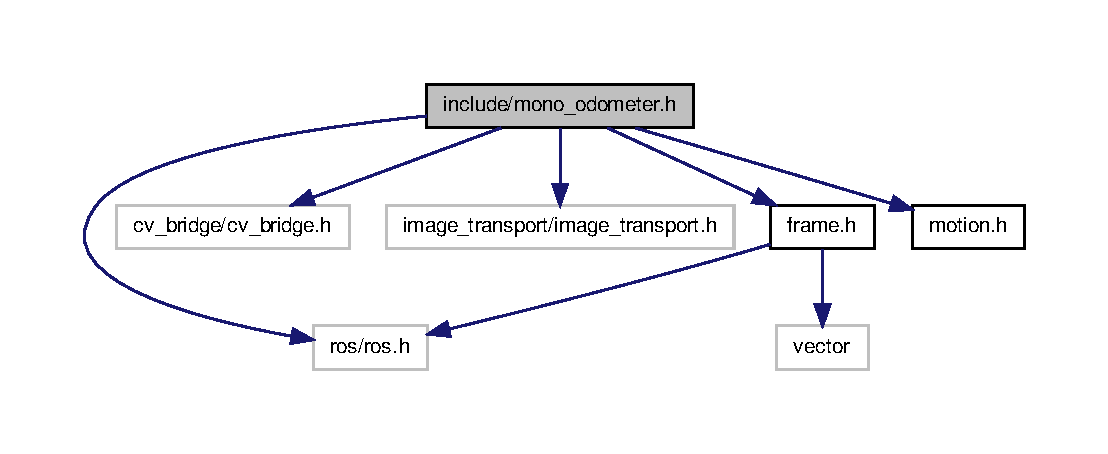
\includegraphics[width=350pt]{mono__odometer_8h__incl}
\end{center}
\end{figure}
\-This graph shows which files directly or indirectly include this file\-:\nopagebreak
\begin{figure}[H]
\begin{center}
\leavevmode
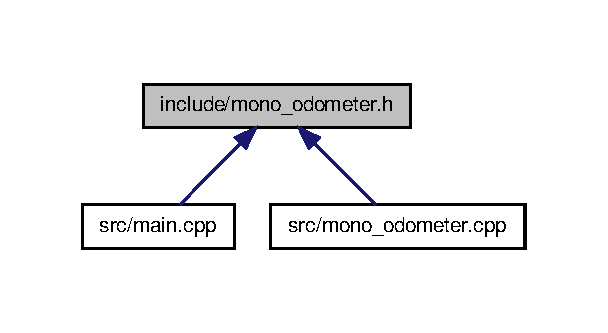
\includegraphics[width=292pt]{mono__odometer_8h__dep__incl}
\end{center}
\end{figure}
\subsection*{\-Classes}
\begin{DoxyCompactItemize}
\item 
class \hyperlink{classLRM_1_1ROSParameter}{\-L\-R\-M\-::\-R\-O\-S\-Parameter}
\item 
class \hyperlink{classLRM_1_1MonoOdometer}{\-L\-R\-M\-::\-Mono\-Odometer}
\end{DoxyCompactItemize}
\subsection*{\-Namespaces}
\begin{DoxyCompactItemize}
\item 
namespace \hyperlink{namespaceLRM}{\-L\-R\-M}
\end{DoxyCompactItemize}

\hypertarget{motion_8h}{\section{include/motion.h \-File \-Reference}
\label{motion_8h}\index{include/motion.\-h@{include/motion.\-h}}
}
\-This graph shows which files directly or indirectly include this file\-:\nopagebreak
\begin{figure}[H]
\begin{center}
\leavevmode
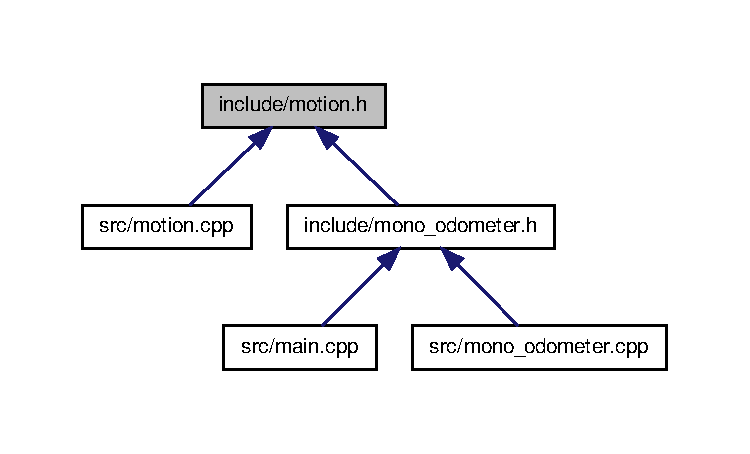
\includegraphics[width=350pt]{motion_8h__dep__incl}
\end{center}
\end{figure}
\subsection*{\-Classes}
\begin{DoxyCompactItemize}
\item 
class \hyperlink{classLRM_1_1Motion}{\-L\-R\-M\-::\-Motion}
\end{DoxyCompactItemize}
\subsection*{\-Namespaces}
\begin{DoxyCompactItemize}
\item 
namespace \hyperlink{namespaceLRM}{\-L\-R\-M}
\end{DoxyCompactItemize}

\hypertarget{feature_8cpp}{\section{src/feature.cpp \-File \-Reference}
\label{feature_8cpp}\index{src/feature.\-cpp@{src/feature.\-cpp}}
}
{\ttfamily \#include \char`\"{}feature.\-h\char`\"{}}\*
\-Include dependency graph for feature.\-cpp\-:\nopagebreak
\begin{figure}[H]
\begin{center}
\leavevmode
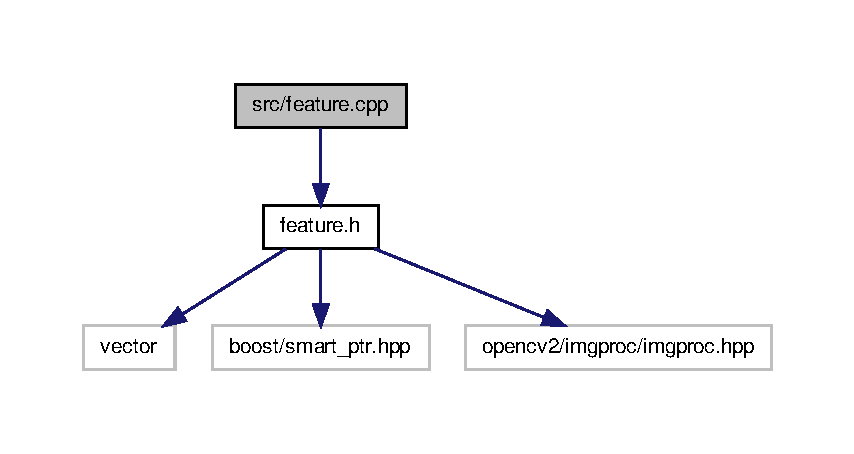
\includegraphics[width=350pt]{feature_8cpp__incl}
\end{center}
\end{figure}
\-This graph shows which files directly or indirectly include this file\-:\nopagebreak
\begin{figure}[H]
\begin{center}
\leavevmode
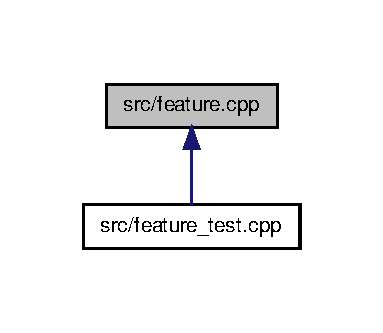
\includegraphics[width=184pt]{feature_8cpp__dep__incl}
\end{center}
\end{figure}
\subsection*{\-Namespaces}
\begin{DoxyCompactItemize}
\item 
namespace \hyperlink{namespaceLRM}{\-L\-R\-M}
\end{DoxyCompactItemize}

\hypertarget{feature__test_8cpp}{\section{src/feature\-\_\-test.cpp \-File \-Reference}
\label{feature__test_8cpp}\index{src/feature\-\_\-test.\-cpp@{src/feature\-\_\-test.\-cpp}}
}
{\ttfamily \#include $<$iostream$>$}\*
{\ttfamily \#include $<$vector$>$}\*
{\ttfamily \#include $<$ros/ros.\-h$>$}\*
{\ttfamily \#include $<$image\-\_\-transport/image\-\_\-transport.\-h$>$}\*
{\ttfamily \#include $<$sensor\-\_\-msgs/\-Image.\-h$>$}\*
{\ttfamily \#include $<$opencv2/imgproc/imgproc.\-hpp$>$}\*
{\ttfamily \#include $<$opencv2/highgui/highgui.\-hpp$>$}\*
{\ttfamily \#include $<$cv\-\_\-bridge/cv\-\_\-bridge.\-h$>$}\*
{\ttfamily \#include \char`\"{}feature.\-cpp\char`\"{}}\*
\-Include dependency graph for feature\-\_\-test.\-cpp\-:\nopagebreak
\begin{figure}[H]
\begin{center}
\leavevmode
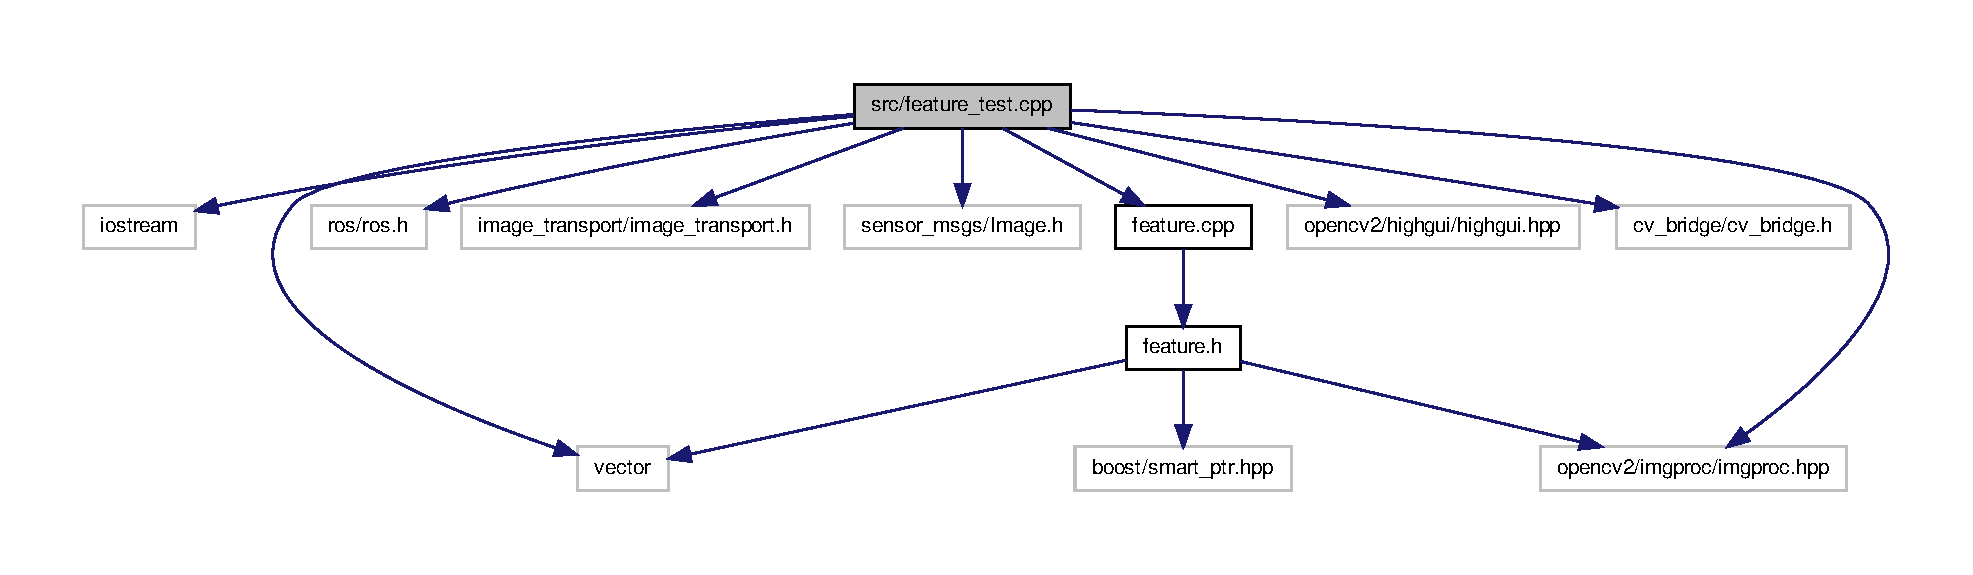
\includegraphics[width=350pt]{feature__test_8cpp__incl}
\end{center}
\end{figure}
\subsection*{\-Functions}
\begin{DoxyCompactItemize}
\item 
void \hyperlink{feature__test_8cpp_a54774dab71cf969f8b85a03bb9741d2d}{\-Image\-Cb} (const sensor\-\_\-msgs\-::\-Image\-Const\-Ptr \&msg)
\item 
int \hyperlink{feature__test_8cpp_a3c04138a5bfe5d72780bb7e82a18e627}{main} (int argc, char $\ast$$\ast$argv)
\end{DoxyCompactItemize}
\subsection*{\-Variables}
\begin{DoxyCompactItemize}
\item 
image\-\_\-transport\-::\-Subscriber \hyperlink{feature__test_8cpp_a58a95828fcf20295c1f5b3a4f6d9974c}{sub}
\item 
image\-\_\-transport\-::\-Publisher \hyperlink{feature__test_8cpp_aa3018a2730fde05a0032471af5d5dff2}{pub}
\end{DoxyCompactItemize}


\subsection{\-Function \-Documentation}
\hypertarget{feature__test_8cpp_a54774dab71cf969f8b85a03bb9741d2d}{\index{feature\-\_\-test.\-cpp@{feature\-\_\-test.\-cpp}!\-Image\-Cb@{\-Image\-Cb}}
\index{\-Image\-Cb@{\-Image\-Cb}!feature_test.cpp@{feature\-\_\-test.\-cpp}}
\subsubsection[{\-Image\-Cb}]{\setlength{\rightskip}{0pt plus 5cm}void {\bf \-Image\-Cb} (
\begin{DoxyParamCaption}
\item[{const sensor\-\_\-msgs\-::\-Image\-Const\-Ptr \&}]{msg}
\end{DoxyParamCaption}
)}}\label{feature__test_8cpp_a54774dab71cf969f8b85a03bb9741d2d}
\-Parameters for \-Shi-\/\-Tomasi algorithm

\-Apply corner detection

\-Draw corners detected \hypertarget{feature__test_8cpp_a3c04138a5bfe5d72780bb7e82a18e627}{\index{feature\-\_\-test.\-cpp@{feature\-\_\-test.\-cpp}!main@{main}}
\index{main@{main}!feature_test.cpp@{feature\-\_\-test.\-cpp}}
\subsubsection[{main}]{\setlength{\rightskip}{0pt plus 5cm}int {\bf main} (
\begin{DoxyParamCaption}
\item[{int}]{argc, }
\item[{char $\ast$$\ast$}]{argv}
\end{DoxyParamCaption}
)}}\label{feature__test_8cpp_a3c04138a5bfe5d72780bb7e82a18e627}
\hyperlink{feature__test_8cpp_a3c04138a5bfe5d72780bb7e82a18e627}{main()} 

\-Here is the call graph for this function\-:\nopagebreak
\begin{figure}[H]
\begin{center}
\leavevmode
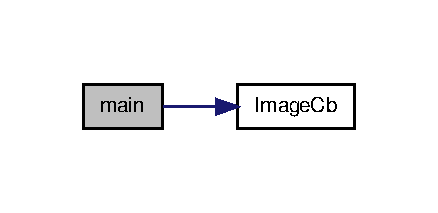
\includegraphics[width=210pt]{feature__test_8cpp_a3c04138a5bfe5d72780bb7e82a18e627_cgraph}
\end{center}
\end{figure}




\subsection{\-Variable \-Documentation}
\hypertarget{feature__test_8cpp_aa3018a2730fde05a0032471af5d5dff2}{\index{feature\-\_\-test.\-cpp@{feature\-\_\-test.\-cpp}!pub@{pub}}
\index{pub@{pub}!feature_test.cpp@{feature\-\_\-test.\-cpp}}
\subsubsection[{pub}]{\setlength{\rightskip}{0pt plus 5cm}image\-\_\-transport\-::\-Publisher {\bf pub}}}\label{feature__test_8cpp_aa3018a2730fde05a0032471af5d5dff2}
\hypertarget{feature__test_8cpp_a58a95828fcf20295c1f5b3a4f6d9974c}{\index{feature\-\_\-test.\-cpp@{feature\-\_\-test.\-cpp}!sub@{sub}}
\index{sub@{sub}!feature_test.cpp@{feature\-\_\-test.\-cpp}}
\subsubsection[{sub}]{\setlength{\rightskip}{0pt plus 5cm}image\-\_\-transport\-::\-Subscriber {\bf sub}}}\label{feature__test_8cpp_a58a95828fcf20295c1f5b3a4f6d9974c}

\hypertarget{frame_8cpp}{\section{src/frame.cpp \-File \-Reference}
\label{frame_8cpp}\index{src/frame.\-cpp@{src/frame.\-cpp}}
}
{\ttfamily \#include \char`\"{}frame.\-h\char`\"{}}\*
\-Include dependency graph for frame.\-cpp\-:
\nopagebreak
\begin{figure}[H]
\begin{center}
\leavevmode
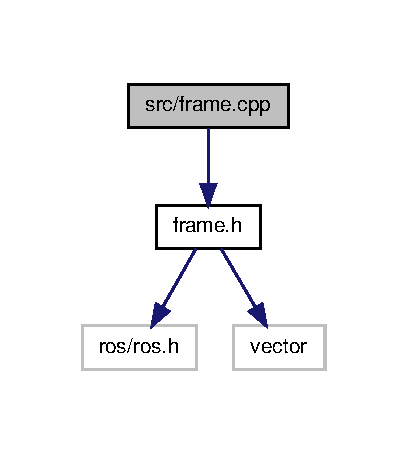
\includegraphics[width=196pt]{frame_8cpp__incl}
\end{center}
\end{figure}
\subsection*{\-Namespaces}
\begin{DoxyCompactItemize}
\item 
namespace \hyperlink{namespaceLRM}{\-L\-R\-M}
\end{DoxyCompactItemize}

\hypertarget{main_8cpp}{\section{src/main.cpp \-File \-Reference}
\label{main_8cpp}\index{src/main.\-cpp@{src/main.\-cpp}}
}
{\ttfamily \#include $<$ros/ros.\-h$>$}\*
{\ttfamily \#include \char`\"{}mono\-\_\-odometer.\-h\char`\"{}}\*
\-Include dependency graph for main.\-cpp\-:\nopagebreak
\begin{figure}[H]
\begin{center}
\leavevmode
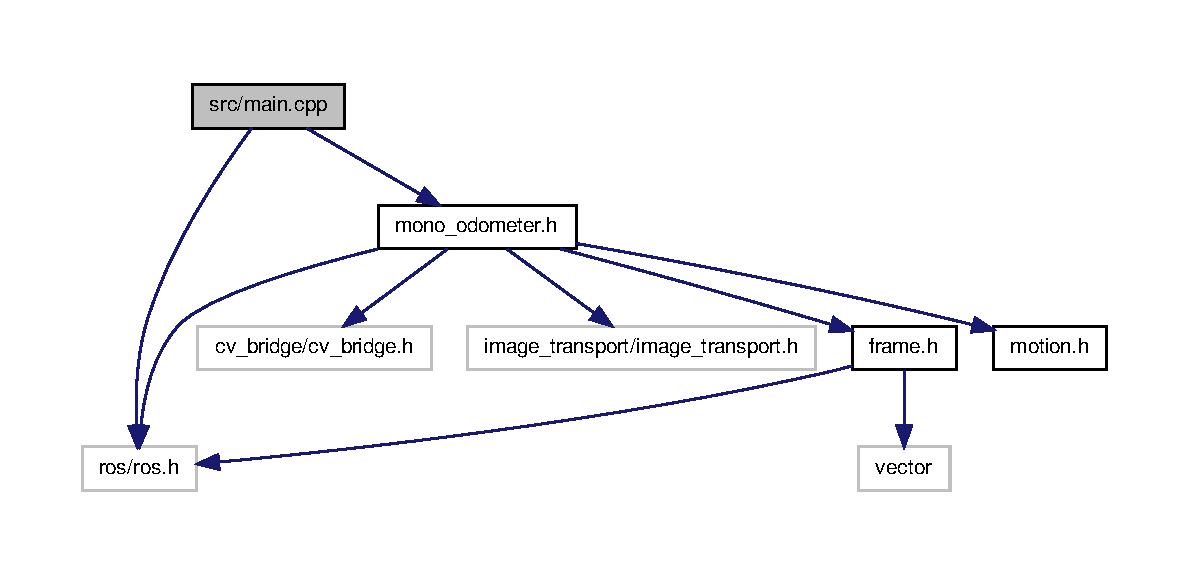
\includegraphics[width=350pt]{main_8cpp__incl}
\end{center}
\end{figure}
\subsection*{\-Functions}
\begin{DoxyCompactItemize}
\item 
int \hyperlink{main_8cpp_a3c04138a5bfe5d72780bb7e82a18e627}{main} (int argc, char $\ast$$\ast$argv)
\end{DoxyCompactItemize}


\subsection{\-Function \-Documentation}
\hypertarget{main_8cpp_a3c04138a5bfe5d72780bb7e82a18e627}{\index{main.\-cpp@{main.\-cpp}!main@{main}}
\index{main@{main}!main.cpp@{main.\-cpp}}
\subsubsection[{main}]{\setlength{\rightskip}{0pt plus 5cm}int {\bf main} (
\begin{DoxyParamCaption}
\item[{int}]{argc, }
\item[{char $\ast$$\ast$}]{argv}
\end{DoxyParamCaption}
)}}\label{main_8cpp_a3c04138a5bfe5d72780bb7e82a18e627}
\hyperlink{main_8cpp_a3c04138a5bfe5d72780bb7e82a18e627}{main()} 
\hypertarget{mono__odometer_8cpp}{\section{src/mono\-\_\-odometer.cpp \-File \-Reference}
\label{mono__odometer_8cpp}\index{src/mono\-\_\-odometer.\-cpp@{src/mono\-\_\-odometer.\-cpp}}
}
{\ttfamily \#include \char`\"{}mono\-\_\-odometer.\-h\char`\"{}}\*
\-Include dependency graph for mono\-\_\-odometer.\-cpp\-:\nopagebreak
\begin{figure}[H]
\begin{center}
\leavevmode
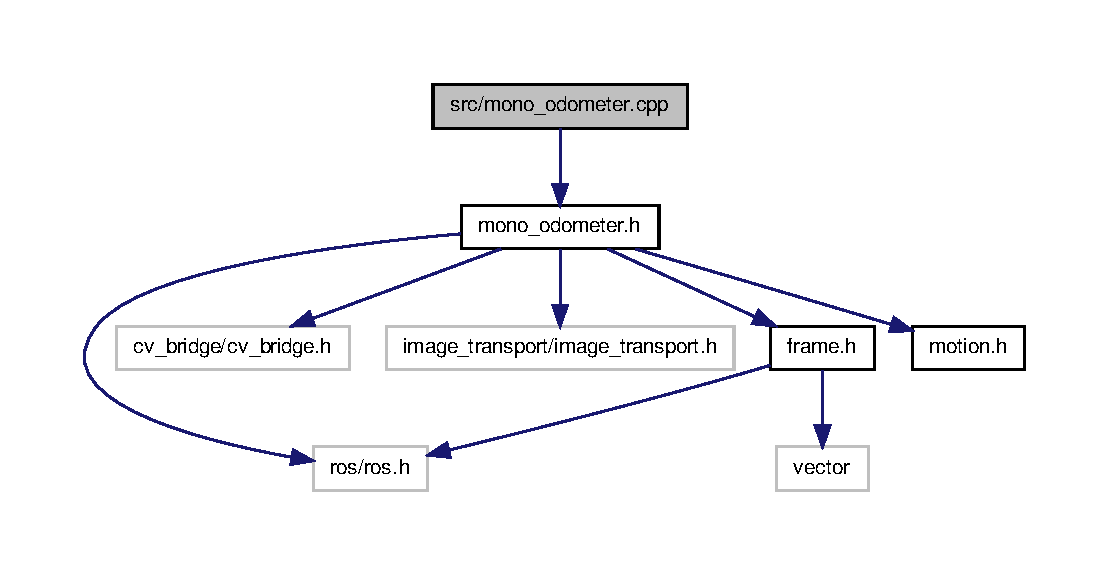
\includegraphics[width=350pt]{mono__odometer_8cpp__incl}
\end{center}
\end{figure}
\subsection*{\-Namespaces}
\begin{DoxyCompactItemize}
\item 
namespace \hyperlink{namespaceLRM}{\-L\-R\-M}
\end{DoxyCompactItemize}

\hypertarget{motion_8cpp}{\section{src/motion.cpp \-File \-Reference}
\label{motion_8cpp}\index{src/motion.\-cpp@{src/motion.\-cpp}}
}
{\ttfamily \#include \char`\"{}motion.\-h\char`\"{}}\*
\-Include dependency graph for motion.\-cpp\-:\nopagebreak
\begin{figure}[H]
\begin{center}
\leavevmode
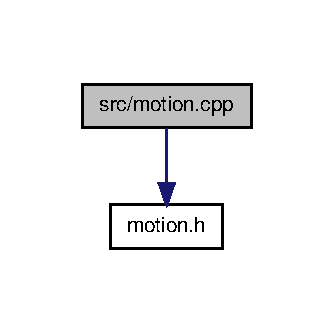
\includegraphics[width=160pt]{motion_8cpp__incl}
\end{center}
\end{figure}
\subsection*{\-Namespaces}
\begin{DoxyCompactItemize}
\item 
namespace \hyperlink{namespaceLRM}{\-L\-R\-M}
\end{DoxyCompactItemize}

\printindex
\end{document}
